\documentclass[aspectratio=169]{beamer}

\usepackage{amsthm}
\usepackage{amssymb}
\usepackage{amsfonts}
\usepackage{amsmath}
\usepackage{mathtools}

\usepackage{pgf}
\usepgflibrary{fpu}
\usepackage{pgfplots}
\usepackage{tikz}
\usetikzlibrary{angles,fit,arrows,calc,math,matrix,intersections,through,backgrounds,cd}
\usepackage{tkz-euclide}
\usepackage{tkz-graph}
\usepackage{graphicx}
\usepackage{hyperref}
\pgfplotsset{compat=1.18}

\usetheme{Pittsburgh}
\usecolortheme{seahorse}

\title{Arithmetic Expression Geometry}
\author[Author] {Mingli Yuan}

\begin{document}
\pgfplotsset{compat=1.18}

\begin{frame}
\maketitle
\end{frame}

\begin{frame}
\frametitle{Table of Contents}
\tableofcontents
\end{frame}

\section{Background, our idea and exploration}

\begin{frame}
    \frametitle{Background, our idea and exploration}
    \begin{enumerate}
        \item Background
        \item Our idea and exploration
    \end{enumerate}
\end{frame}

\begin{frame}
    \frametitle{Background}
    \begin{figure}[ht]\centering
    \resizebox{0.5\textwidth}{!}{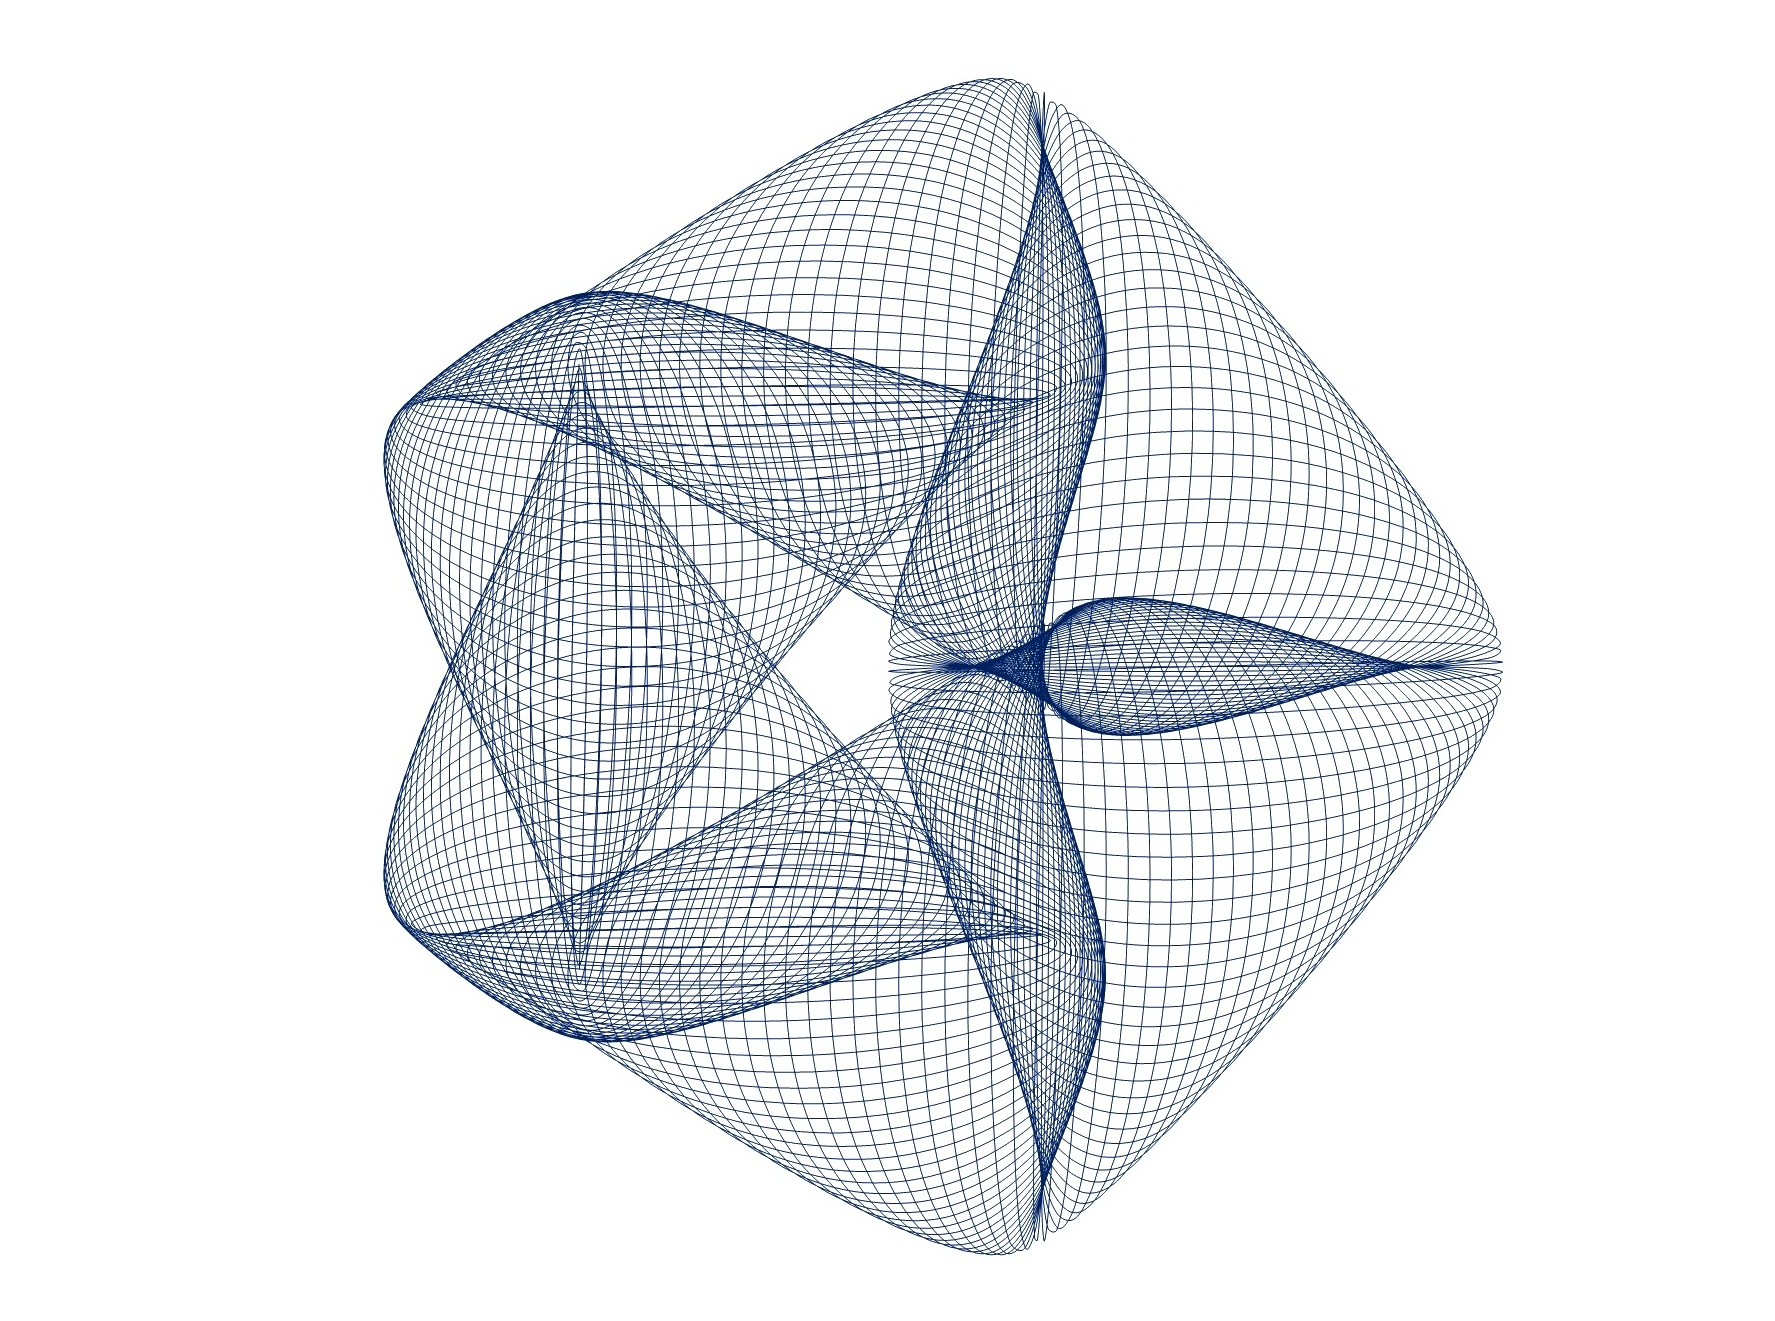
\includegraphics{../images/param_curve}}
    \end{figure}
\end{frame}

\begin{frame}
    \frametitle{How to describe a change over time?}
    \begin{columns}
        \begin{column}{0.7\textwidth}
            Two methods to describe a small change over time:
            \begin{itemize}
                \item by quantity: adding a small near-zero amount of quantity
                \item by ratio: multiplying a near-unit ratio
            \end{itemize}
            Traditional calculus is based on the first method, Riemann integral is additive.
            We can use functions $\exp$ and $\log$ to convert between the two methods.
        \end{column}
        \begin{column}{0.3\textwidth}
            \begin{figure}[ht]\centering
            \resizebox{1.0\textwidth}{!}{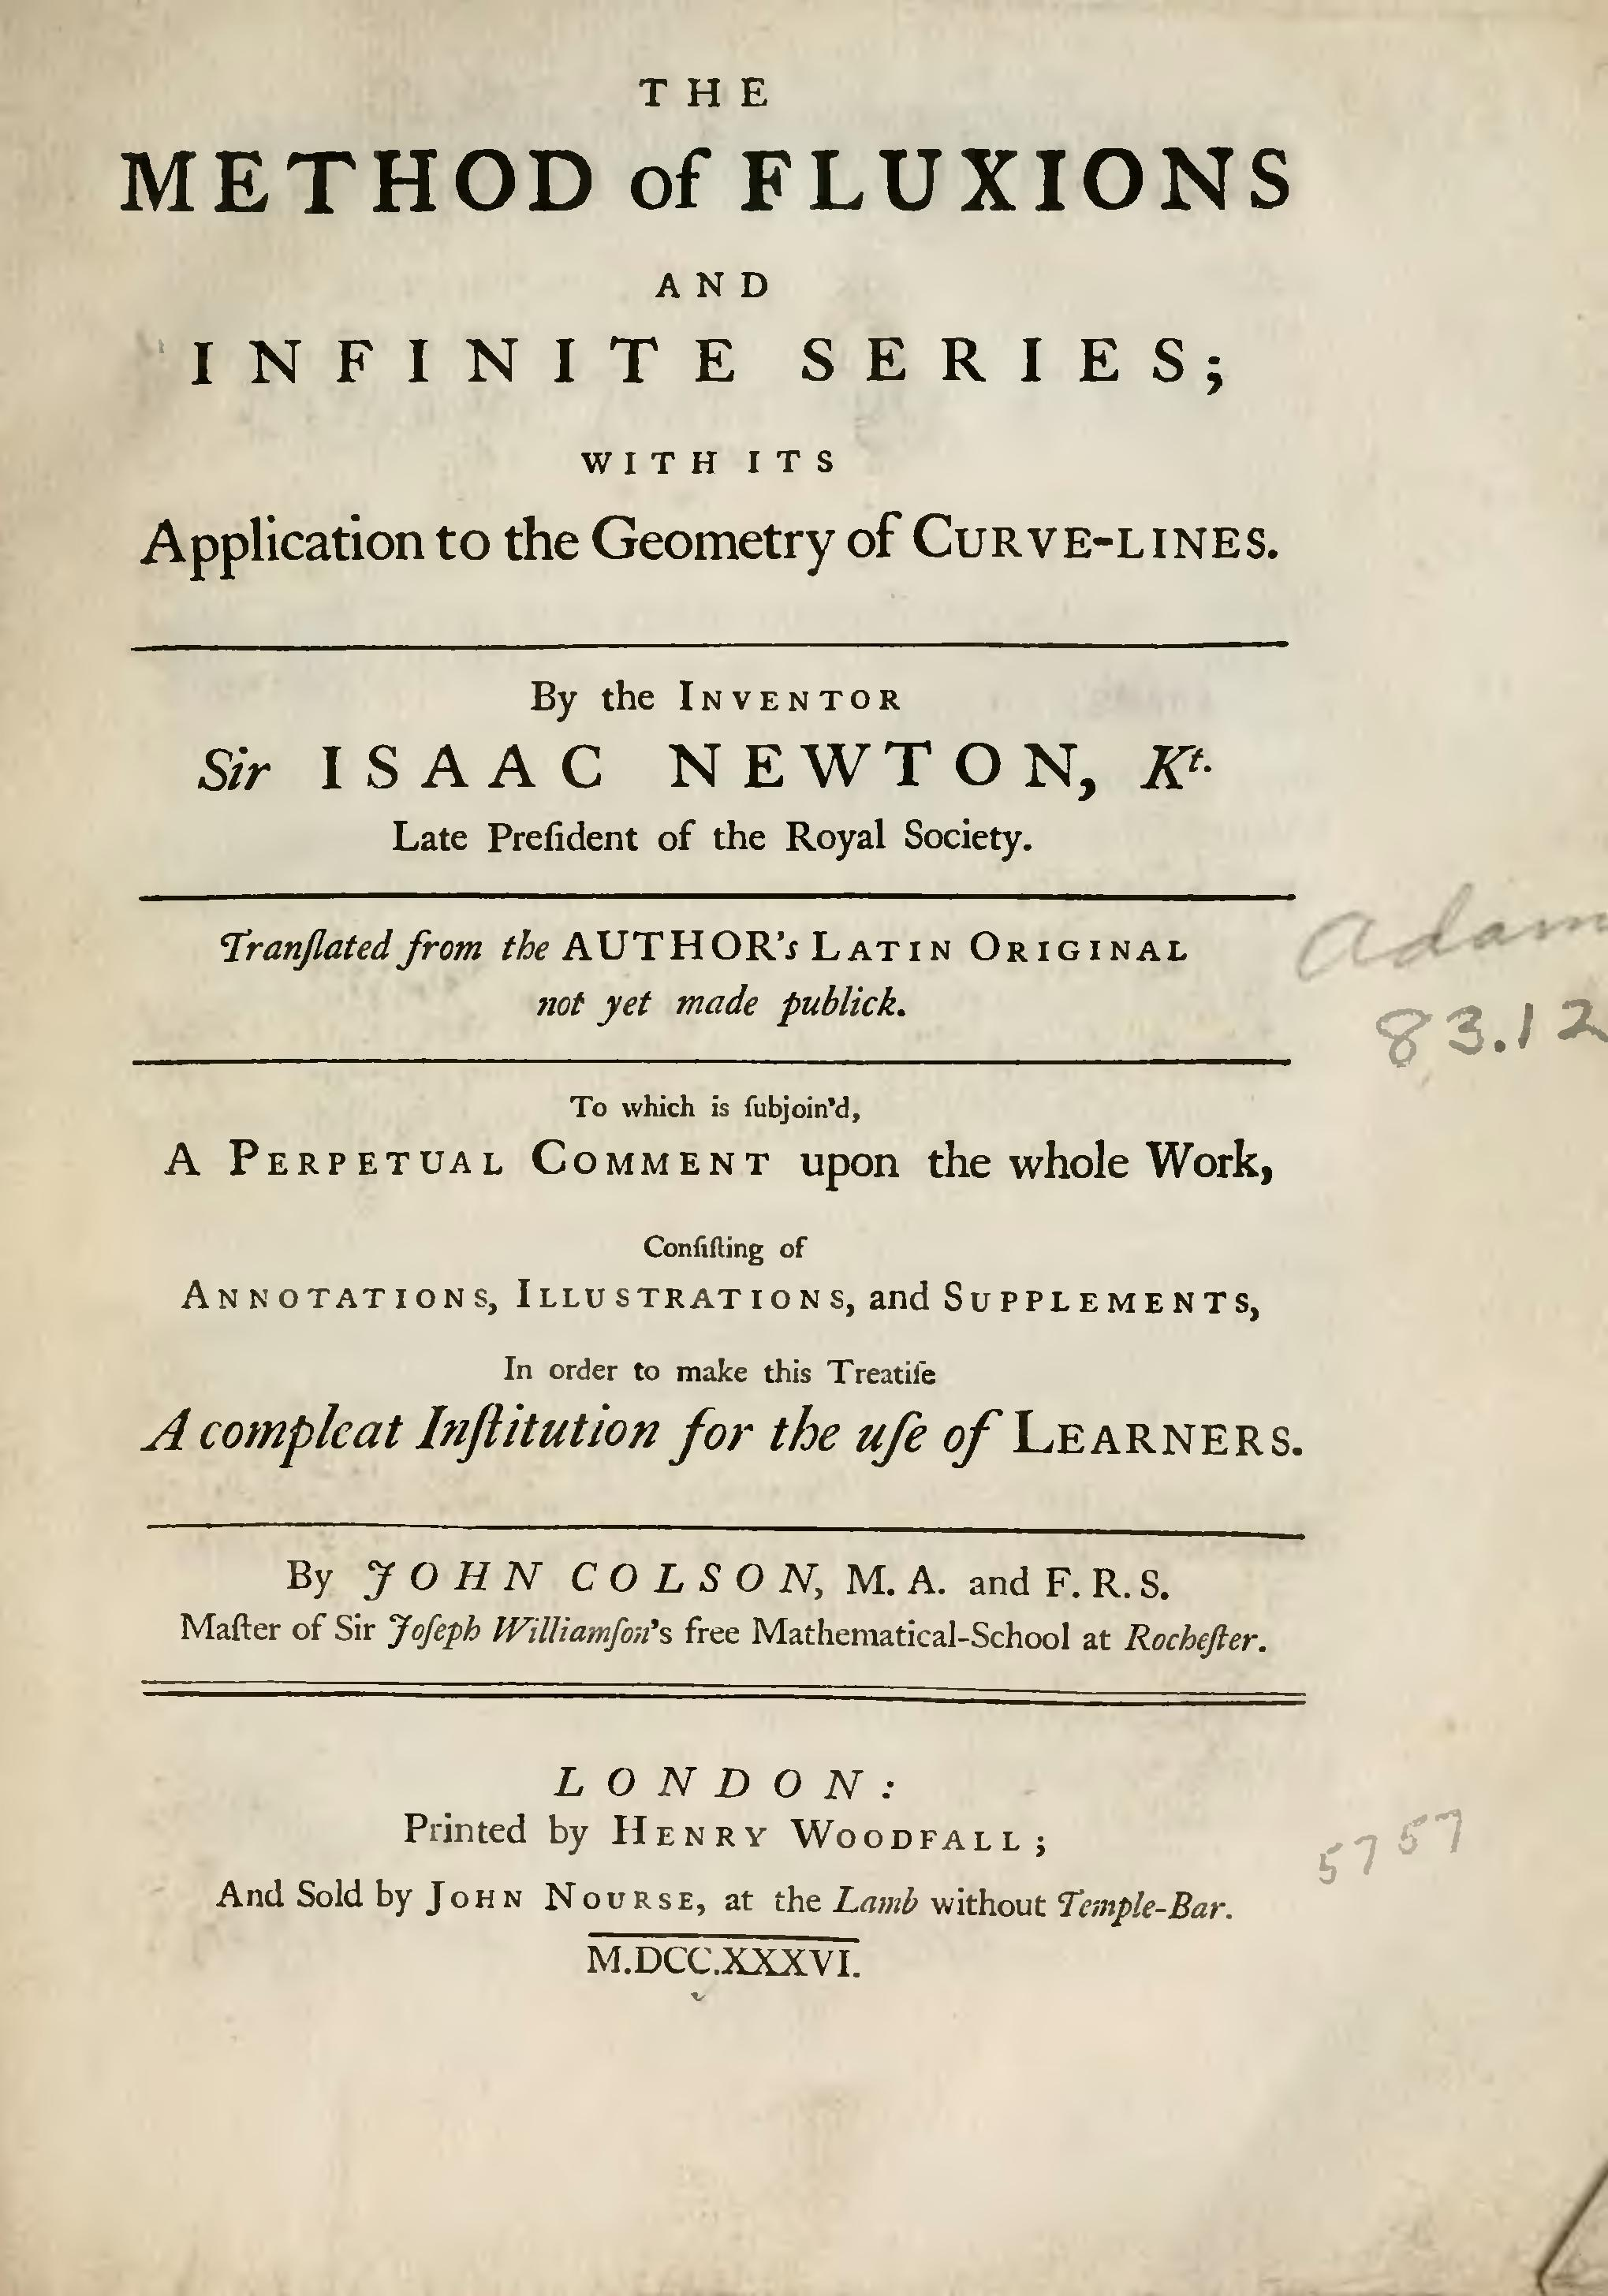
\includegraphics{../images/fluxions}}
            \caption{Method of Fluxions}
            \end{figure}
        \end{column}
    \end{columns}
\end{frame}

\begin{frame}
    \frametitle{Product integration}
    \begin{columns}
            \begin{column}{0.3\textwidth}
                \begin{figure}[ht]\centering
                \resizebox{1.0\textwidth}{!}{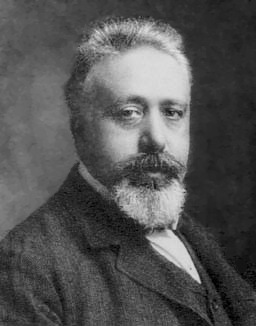
\includegraphics{../images/vito_volterra}}
                \caption{Vito Volterra}
                \end{figure}
            \end{column}
            \begin{column}{0.7\textwidth}
            Matrix-valued non-commutative derivative and integration, left and right
            \begin{itemize}
                \item $\frac{d}{dx} A(x) = \lim_{\Delta x \to 0} \frac{A(x + \Delta x) A^{-1}(x) - I}{\Delta x}$
                \item $A(x) \frac{d}{dx} = \lim_{\Delta x \to 0} \frac{A^{-1}(x) A(x + \Delta x) - I}{\Delta x}$
                \item $\prod_{a}^{b} (I + A(x) dx) = \lim_{\nu(P) \to 0} \prod_{i=m}^{1}(I + A(\xi_i))$
                \item $(I + A(x) dx) \prod_{a}^{b}  = \lim_{\nu(P) \to 0} \prod_{i=1}^{m}(I + A(\xi_i))$
            \end{itemize}
            An interesting formula connect product integration and normal additive integration
            $\prod_a^b (I + A(x) dx) = I + \int_a^b A(x) dx + \int_a^b \int_a^x A(x) A(y) dy dx + \cdots$
            \end{column}
    \end{columns}
\end{frame}

\begin{frame}
    \frametitle{How about mixing up additive and multiplicative steps?}
    Question: How about mixing additive and multiplicative steps up in one process?

    We can get a first order non-homogeneous differential equation
    $$ \frac{dx}{dt} = (1 + f(t)) x + g(t) $$
\end{frame}

\begin{frame}
    \frametitle{Our idea and exploration}
    \begin{figure}[ht]\centering
    \resizebox{0.5\textwidth}{!}{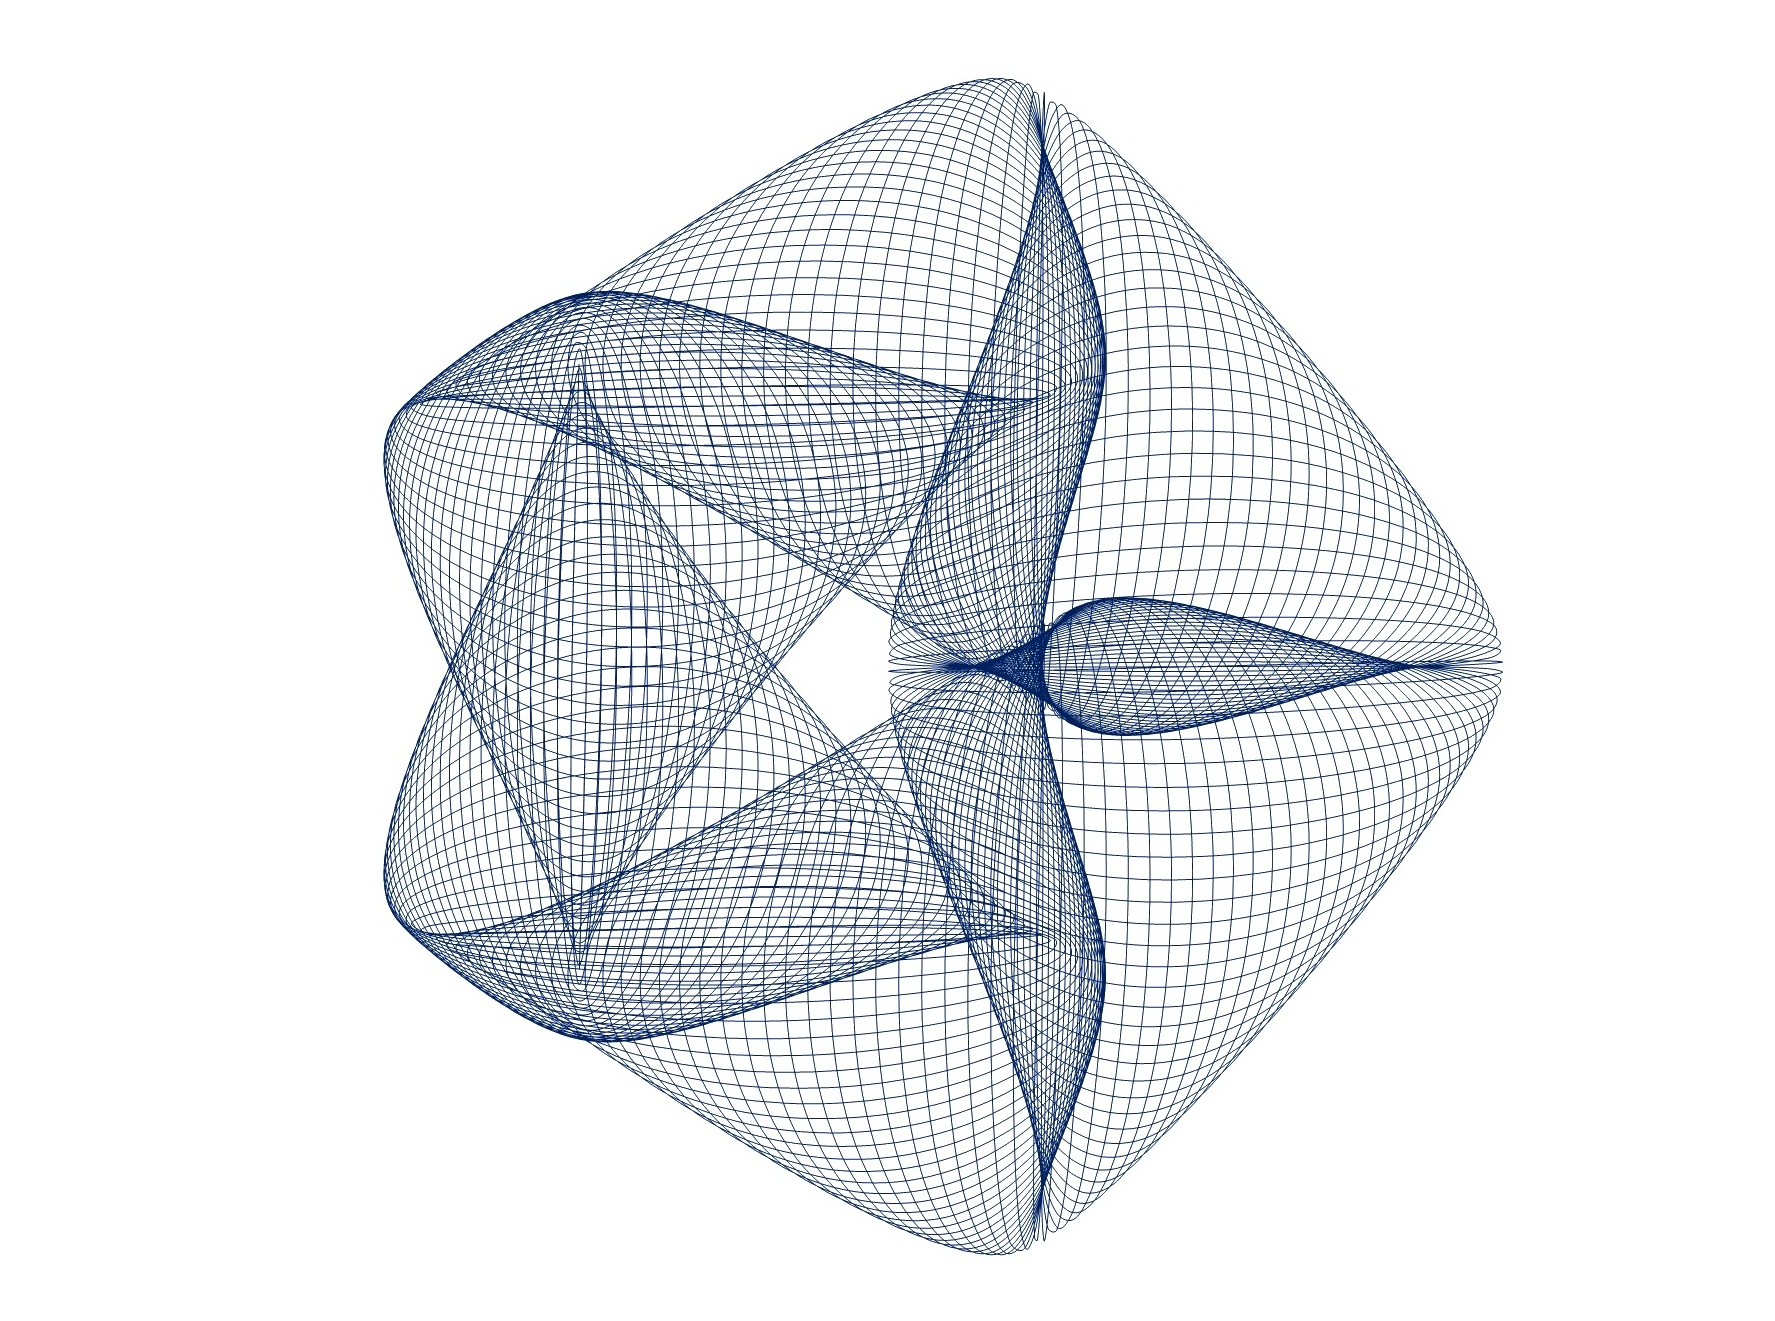
\includegraphics{../images/param_curve}}
    \end{figure}
\end{frame}

\begin{frame}
\frametitle{Regularity of word2vec}
The famous example of word2vec
\begin{figure}[ht]
\centering
\resizebox{0.5\textwidth}{!}{
\begin{tikzpicture}[x=0.5cm,y=0.5cm,z=0.3cm,>=stealth]
\draw[->] (xyz cs:x=-7.0) -- (xyz cs:x=7.0) node[above] {$x_0$};
\draw[->] (xyz cs:y=0) -- (xyz cs:y=7.0) node[right] {$x_n$};
\draw[->] (xyz cs:z=-7.0) -- (xyz cs:z=7.0) node[above] {$x_i$};

\node[fill,circle,inner sep=1.5pt,label={left:$king$}] (p) at (xyz cs:x=-3.0, y=3.0, z=-3.0) {};
\node[fill,circle,inner sep=1.5pt,label={right:$man$}] (q) at (xyz cs:x=2.0, y=-3.0, z=3.0) {};
\node[fill,circle,inner sep=1.5pt,label={left:$queen$}] (r) at (xyz cs:x=-3.0, y=3.0, z=3.0) {};
\node[fill,circle,inner sep=1.5pt,label={right:$woman$}] (s) at (xyz cs:x=2.0, y=-3.0, z=9.0) {};
\draw[dashed, blue] (p) -- (q);
\draw[dashed, blue] (r) -- (s);
\draw[dashed, red] (p) -- (r);
\draw[dashed, red] (q) -- (s);
\end{tikzpicture}
}
\caption{regulairty of word2vec}
\label{fig:regulairty-of-word2vec}
\end{figure}
\end{frame}

\begin{frame}
\frametitle{The case of numbers}
\[
(\alpha + 1) \times 2 \neq \alpha \times 2 + 1
\]

\begin{figure}[ht]
\centering
\resizebox{0.5\textwidth}{!}{
\begin{tikzpicture}[x=0.5cm,y=0.5cm,z=0.3cm,>=stealth]
\draw[->] (xyz cs:x=-7.0) -- (xyz cs:x=7.0) node[right] {$x_0$};
\draw[->] (xyz cs:y=0) -- (xyz cs:y=7.0) node[right] {$x_n$};
\draw[->] (xyz cs:z=-7.0) -- (xyz cs:z=7.0) node[above] {$x_i$};

\node[fill,circle,inner sep=1.5pt,label={left:$\alpha$}] (p) at (xyz cs:x=-3.0, y=3.0, z=-3.0) {};
\node[fill,circle,inner sep=1.5pt,label={right:$\alpha+1$}] (q) at (xyz cs:x=2.0, y=-3.0, z=3.0) {};
\node[fill,circle,inner sep=1.5pt,label={left:$\alpha \times 2$}] (r) at (xyz cs:x=-3.0, y=3.0, z=3.0) {};
\node[fill,circle,inner sep=1.5pt,label={right:$(\alpha + 1) \times 2 \neq \alpha \times 2 + 1$}] (s) at (xyz cs:x=2.0, y=-3.0, z=9.0) {};
\draw[dashed, blue] (p) -- (q);
\draw[dashed, blue] (r) -- (s);
\draw[dashed, red] (p) -- (r);
\draw[dashed, red] (q) -- (s);
\end{tikzpicture}
}
\caption{contradiction of numbers in Euclidean space}
\label{fig:contradiction-of-numbers}
\end{figure}

\end{frame}

\begin{frame}
\frametitle{One arrangement in hyperbolic space}
\begin{figure}[ht]\centering
\resizebox{0.5\textwidth}{!}{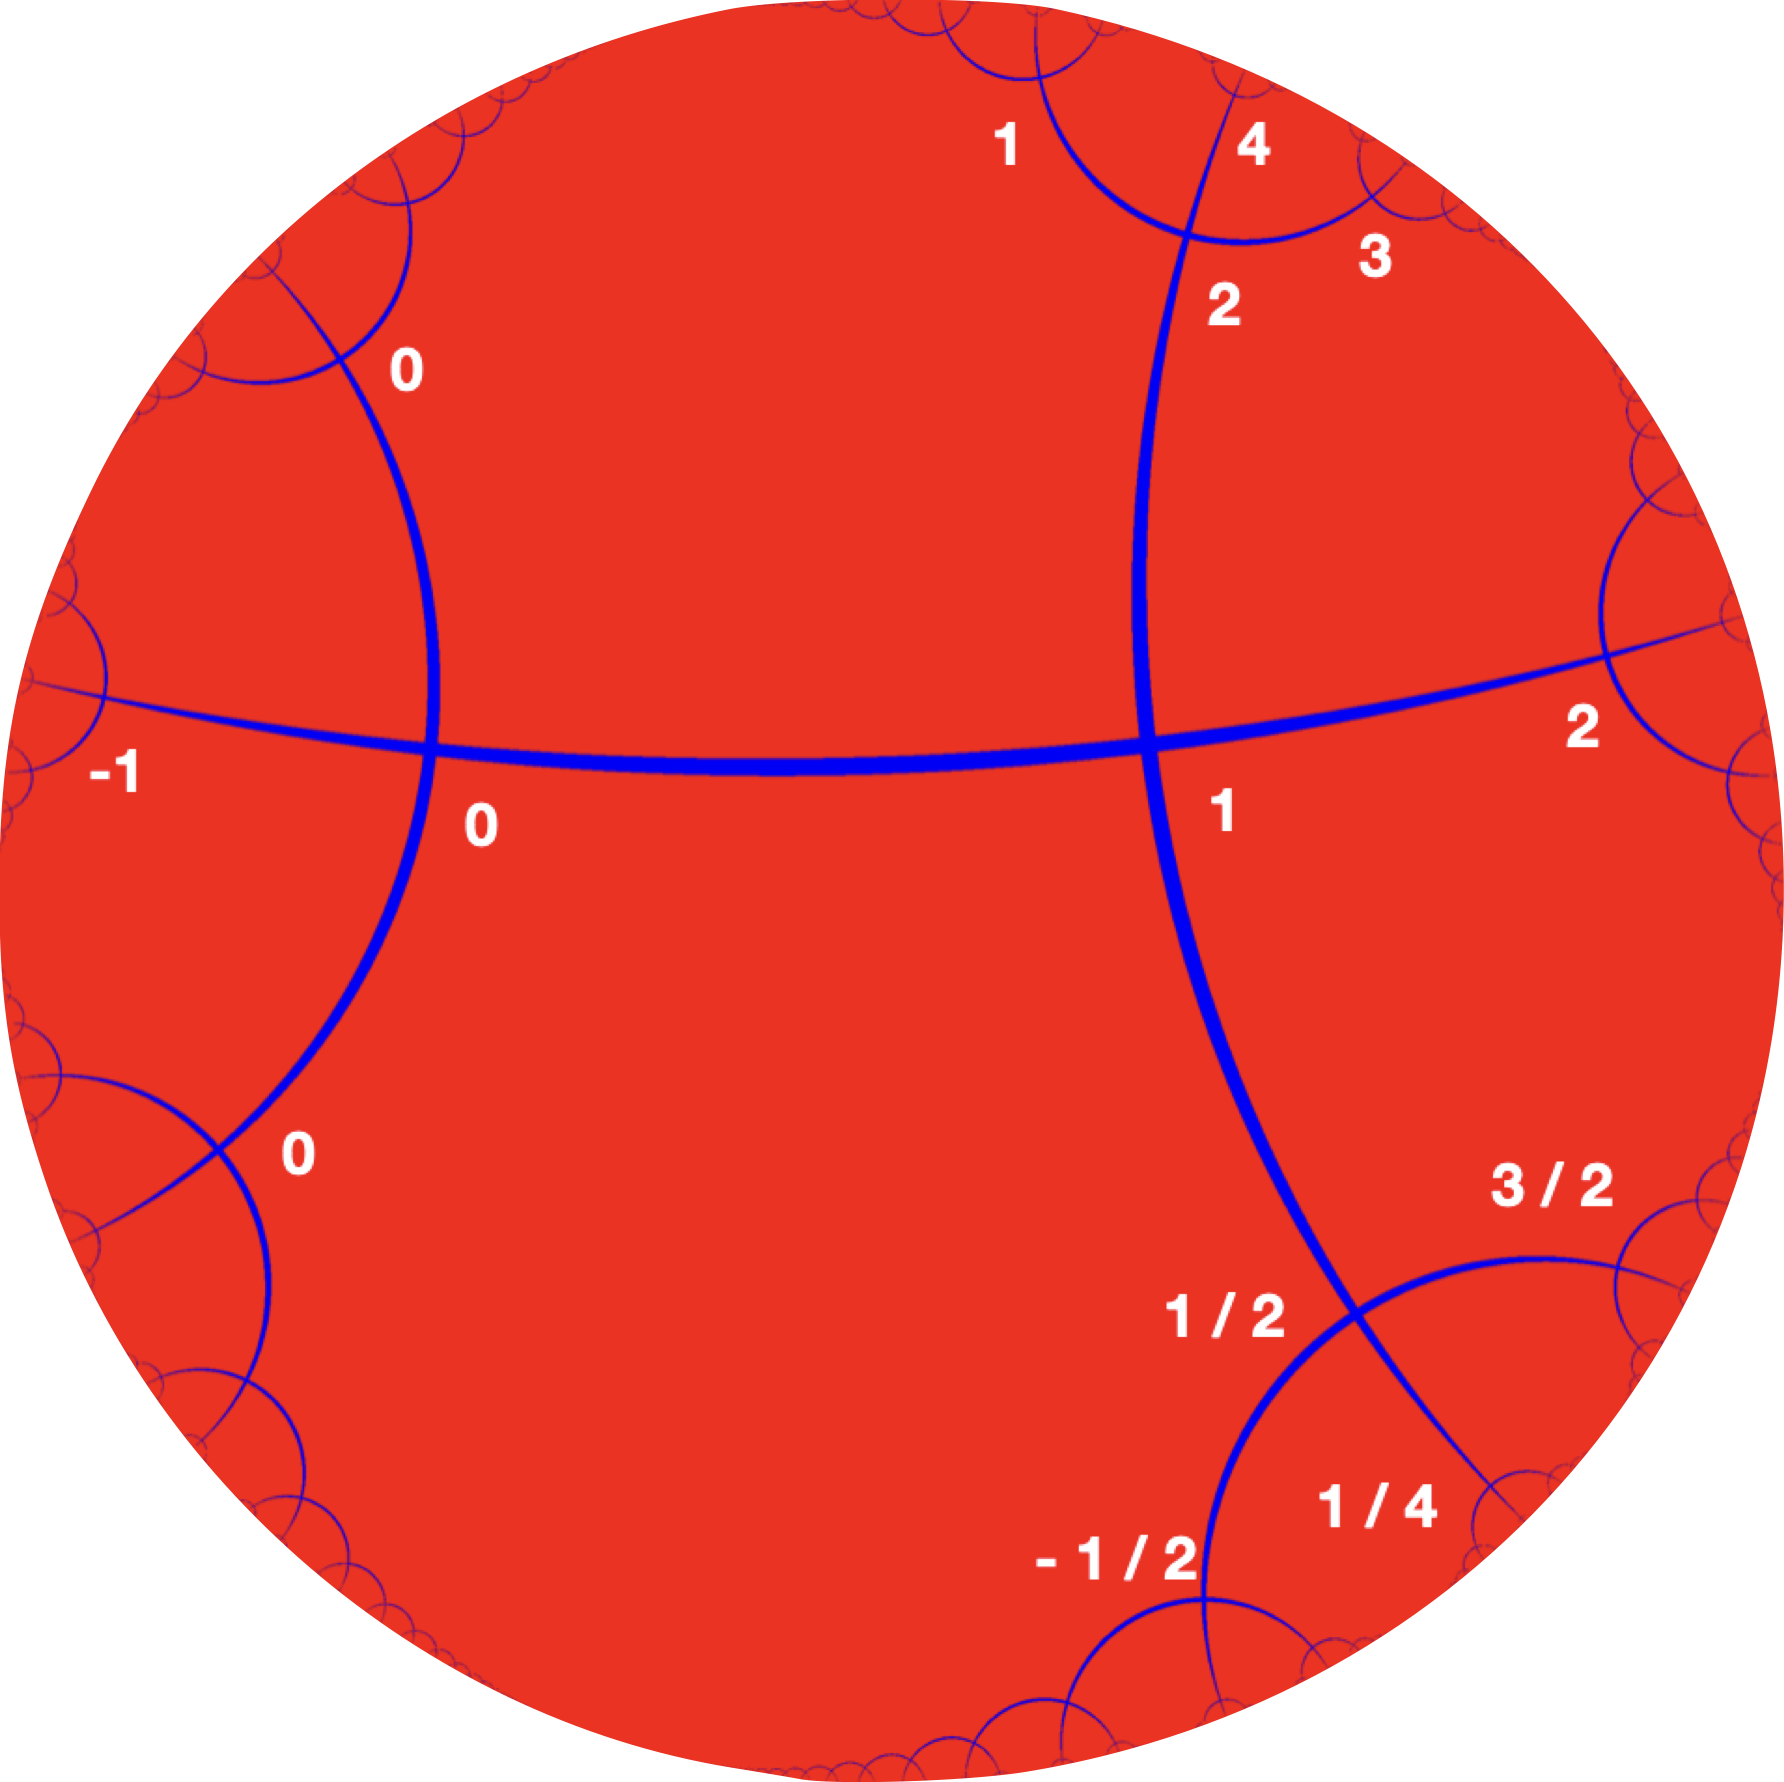
\includegraphics{../images/assignment2}}
\end{figure}
\end{frame}

\begin{frame}
    \frametitle{The flow equation}

    Suppose we have a base point $a_0$, and we step a small distance away from $a_0$.

    Addition first

    \[
        a_{\delta} = (a_0 + \mu \epsilon \cos \theta)e^{\lambda \epsilon \sin \theta}
    \]

    Multiplication first

    \[
        a_{\delta} = a_0 e^{\lambda \epsilon \sin \theta} + \mu \epsilon \cos \theta
    \]

\end{frame}

\begin{frame}
    \frametitle{The flow equation}

    Both formula can be simplified to the same result:

    \[
        a_{\delta} = a_0 + \epsilon (a_0 \lambda \sin \theta + \mu \cos \theta)
    \]

    Then, we have the following equation:

    \[
        \frac{1}{\delta} (a_{\delta} - a_0) = \frac{\epsilon}{\delta} (\mu \cos \theta + a_0 \lambda \sin \theta)
    \]

    When both $\delta$ and $\epsilon$ are towards zero, we get $da / dt$, and hence

    \[
        \frac{da}{dt} = u (\mu \cos \theta + a \lambda \sin \theta)
    \]

    Or, we can change it to another form

    \begin{equation}
        \frac{da}{ds} = \mu \cos \theta + a \lambda \sin \theta\label{eq:flow}
    \end{equation}

\end{frame}

\begin{frame}
    \frametitle{Embeding of discrete grid}
    The flow equation can be solved formally
    \[
        \frac{da}{ds} = \mu \cos \theta + a \lambda \sin \theta
    \]
    and the formal solution is
    \begin{equation}\label{eq:directformalsolution}
    a =  a_0 e^{\lambda s \sin \theta} + \frac{\mu}{\lambda} (e^{\lambda s \sin \theta} - 1) \cot \theta
    \end{equation}

    \[
        a = a_0 e^{\lambda s \sin \theta} + \mu s \cos \theta + \frac{\mu}{2\lambda} \sin 2\theta (\frac{\lambda^2s^2}{2!} + \frac{\lambda^3s^3}{3!} \sin \theta + \frac{\lambda^4s^4}{4!} \sin^2 \theta + \cdots)
    \]

    \[
        a = a_0 e^{\lambda s \sin \theta} + \mu s \cos \theta + \frac{\mu}{2\lambda} \Psi(s) \sin 2\theta
    \]

    So $\theta = 2k\pi$ encode addition, $\theta = 2k\pi + \frac{\pi}{2}$ encode multiplication,
    and $\theta = 2k\pi + \pi$ encode subtraction, and $\theta = 2k\pi + \frac{3\pi}{2}$ encode division.
\end{frame}

\begin{frame}
\frametitle{Another arrangement in hyperbolic space}

\[
    a = - \frac{x}{y}
\]

\begin{figure}[ht]
\centering
\resizebox{0.7\textwidth}{!}{
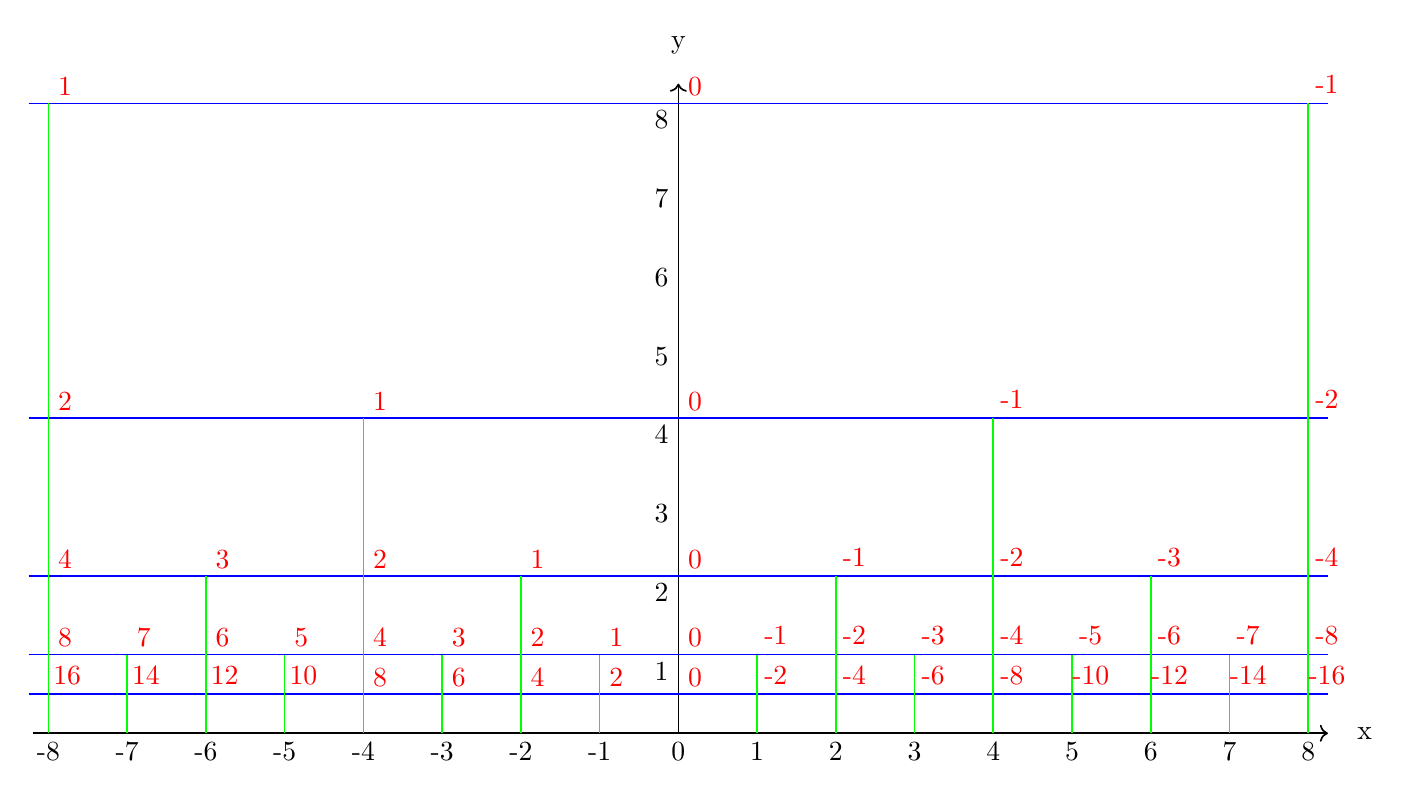
\begin{tikzpicture}
\draw [black, line width=0.6pt, ->] (0,0) to[out=90,in=270] (0,8.25);
\node [anchor=south] at (0,8.5) {y};
\draw [black, line width=0.6pt, ->] (-8.2,0) to[out=0,in=180] (8.25,0);
\node [anchor=west] at (8.5,0) {x};
\foreach \x in {-8,-7,-6,-5,-4,-3,-2,-1,0,1,2,3,4,5,6,7,8}
  \node [anchor=north] at (\x,0) {\x};
\foreach \y in {1,2,3,4,5,6,7,8}
  \node [anchor=45] at (0,\y) {\y};

\draw [blue, line width=0.6pt] (-8.25,0.5) to[out=0,in=180] (8.25,0.5);
\draw [blue, line width=0.6pt] (-8.25,1) to[out=0,in=180] (8.25,1);
\draw [blue, line width=0.6pt] (-8.25,2) to[out=0,in=180] (8.25,2);
\draw [blue, line width=0.6pt] (-8.25,4) to[out=0,in=180] (8.25,4);
\draw [blue, line width=0.6pt] (-8.25,8) to[out=0,in=180] (8.25,8);

\draw [green, line width=0.6pt] (-8,0) to[out=90,in=270] (-8,1);
\draw [green, line width=0.6pt] (-7,0) to[out=90,in=270] (-7,1);
\draw [green, line width=0.6pt] (-6,0) to[out=90,in=270] (-6,1);
\draw [green, line width=0.6pt] (-5,0) to[out=90,in=270] (-5,1);
\draw [green, line width=0.6pt] (-4,0) to[out=90,in=270] (-4,1);
\draw [green, line width=0.6pt] (-3,0) to[out=90,in=270] (-3,1);
\draw [green, line width=0.6pt] (-2,0) to[out=90,in=270] (-2,1);
\draw [green, line width=0.6pt] (-1,0) to[out=90,in=270] (-1,1);
\draw [green, line width=0.6pt] (1,0) to[out=90,in=270] (1,1);
\draw [green, line width=0.6pt] (2,0) to[out=90,in=270] (2,1);
\draw [green, line width=0.6pt] (3,0) to[out=90,in=270] (3,1);
\draw [green, line width=0.6pt] (4,0) to[out=90,in=270] (4,1);
\draw [green, line width=0.6pt] (5,0) to[out=90,in=270] (5,1);
\draw [green, line width=0.6pt] (6,0) to[out=90,in=270] (6,1);
\draw [green, line width=0.6pt] (7,0) to[out=90,in=270] (7,1);
\draw [green, line width=0.6pt] (8,0) to[out=90,in=270] (8,1);

\draw [green, line width=0.6pt] (-8,1) to[out=90,in=270] (-8,2);
\draw [green, line width=0.6pt] (-6,1) to[out=90,in=270] (-6,2);
\draw [green, line width=0.6pt] (-4,1) to[out=90,in=270] (-4,2);
\draw [green, line width=0.6pt] (-2,1) to[out=90,in=270] (-2,2);
\draw [green, line width=0.6pt] (2,1) to[out=90,in=270] (2,2);
\draw [green, line width=0.6pt] (4,1) to[out=90,in=270] (4,2);
\draw [green, line width=0.6pt] (6,1) to[out=90,in=270] (6,2);
\draw [green, line width=0.6pt] (8,1) to[out=90,in=270] (8,2);

\draw [green, line width=0.6pt] (-8,2) to[out=90,in=270] (-8,4);
\draw [green, line width=0.6pt] (-4,2) to[out=90,in=270] (-4,4);
\draw [green, line width=0.6pt] (4,2) to[out=90,in=270] (4,4);
\draw [green, line width=0.6pt] (8,2) to[out=90,in=270] (8,4);

\draw [green, line width=0.6pt] (-8,4) to[out=90,in=270] (-8,8);
\draw [green, line width=0.6pt] (8,4) to[out=90,in=270] (8,8);

\node [anchor=225, red] at (-8,0.5) {16};
\node [anchor=225, red] at (-7,0.5) {14};
\node [anchor=225, red] at (-6,0.5) {12};
\node [anchor=225, red] at (-5,0.5) {10};
\node [anchor=225, red] at (-4,0.5) {8};
\node [anchor=225, red] at (-3,0.5) {6};
\node [anchor=225, red] at (-2,0.5) {4};
\node [anchor=225, red] at (-1,0.5) {2};
\node [anchor=225, red] at (0,0.5) {0};
\node [anchor=225, red] at (1,0.5) {-2};
\node [anchor=225, red] at (2,0.5) {-4};
\node [anchor=225, red] at (3,0.5) {-6};
\node [anchor=225, red] at (4,0.5) {-8};
\node [anchor=225, red] at (5,0.5) {-10};
\node [anchor=225, red] at (6,0.5) {-12};
\node [anchor=225, red] at (7,0.5) {-14};
\node [anchor=225, red] at (8,0.5) {-16};

\node [anchor=225, red] at (-8,1) {8};
\node [anchor=225, red] at (-7,1) {7};
\node [anchor=225, red] at (-6,1) {6};
\node [anchor=225, red] at (-5,1) {5};
\node [anchor=225, red] at (-4,1) {4};
\node [anchor=225, red] at (-3,1) {3};
\node [anchor=225, red] at (-2,1) {2};
\node [anchor=225, red] at (-1,1) {1};
\node [anchor=225, red] at (0,1) {0};
\node [anchor=225, red] at (1,1) {-1};
\node [anchor=225, red] at (2,1) {-2};
\node [anchor=225, red] at (3,1) {-3};
\node [anchor=225, red] at (4,1) {-4};
\node [anchor=225, red] at (5,1) {-5};
\node [anchor=225, red] at (6,1) {-6};
\node [anchor=225, red] at (7,1) {-7};
\node [anchor=225, red] at (8,1) {-8};

\node [anchor=225, red] at (-8,2) {4};
\node [anchor=225, red] at (-6,2) {3};
\node [anchor=225, red] at (-4,2) {2};
\node [anchor=225, red] at (-2,2) {1};
\node [anchor=225, red] at (0,2) {0};
\node [anchor=225, red] at (2,2) {-1};
\node [anchor=225, red] at (4,2) {-2};
\node [anchor=225, red] at (6,2) {-3};
\node [anchor=225, red] at (8,2) {-4};

\node [anchor=225, red] at (-8,4) {2};
\node [anchor=225, red] at (-4,4) {1};
\node [anchor=225, red] at (0,4) {0};
\node [anchor=225, red] at (4,4) {-1};
\node [anchor=225, red] at (8,4) {-2};

\node [anchor=225, red] at (-8,8) {1};
\node [anchor=225, red] at (0,8) {0};
\node [anchor=225, red] at (8,8) {-1};

\end{tikzpicture}
}
\label{fig:gridex0}
\end{figure}
\end{frame}

\begin{frame}
    \frametitle{Encoding threadlike expressions as paths}

    \begin{itemize}
        \item black line $1 \times 8 - 5 = 3$
        \item purple line $(1 - \frac{5}{8}) \times 8 = 3$
        \item orange line: a speical integration
    \end{itemize}

    \begin{figure}[ht]
        \centering
        \resizebox{0.6\textwidth}{!}{
            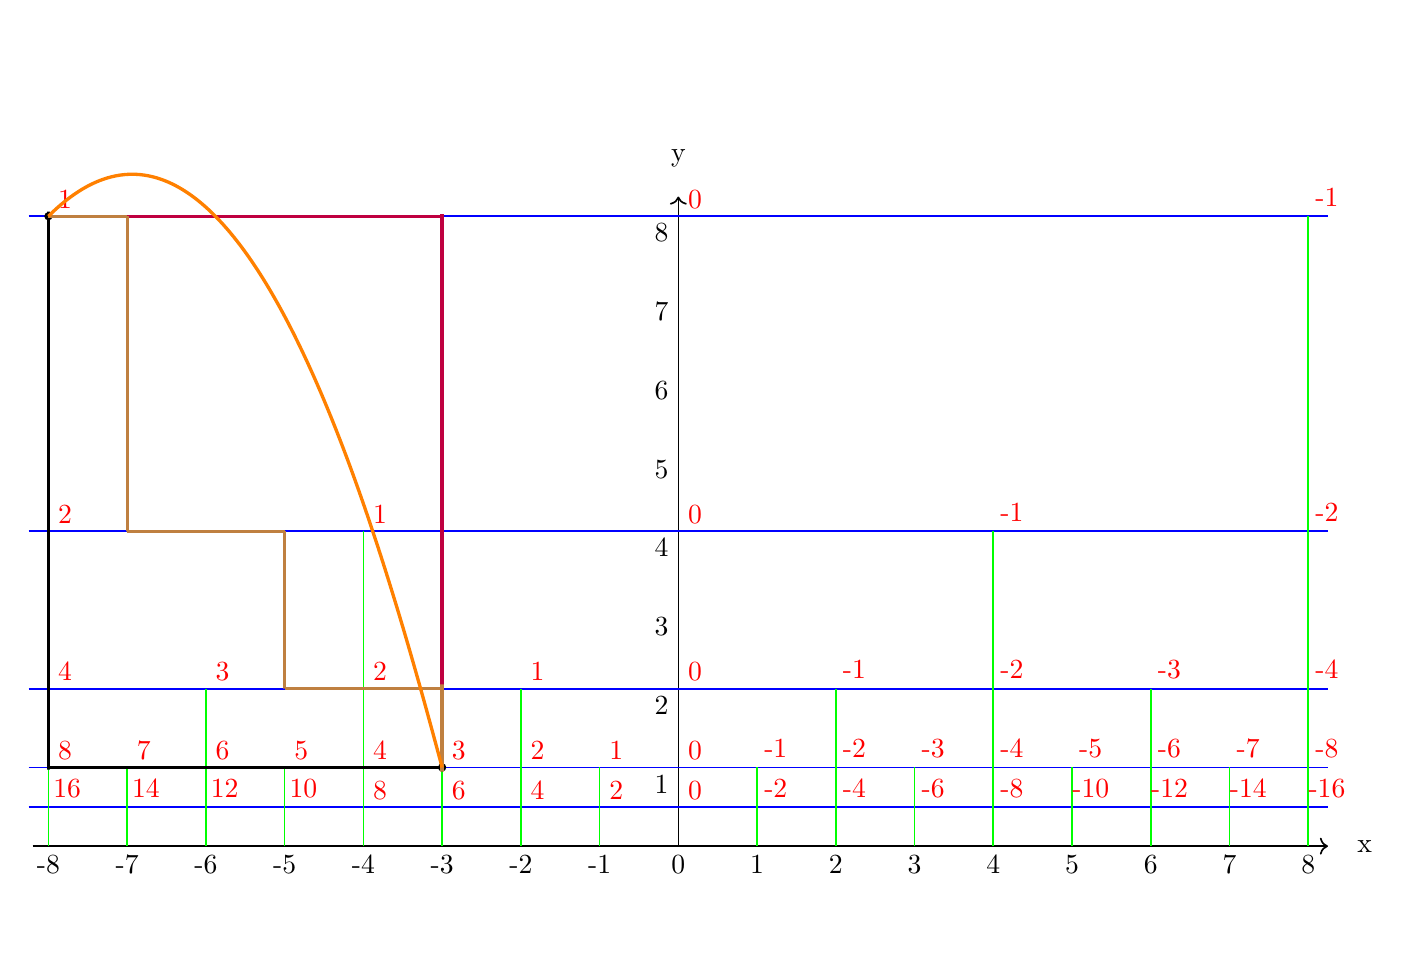
\begin{tikzpicture}
                \draw [black, line width=0.6pt, ->] (0,0) to[out=90,in=270] (0,8.25);
                \node [anchor=south] at (0,8.5) {y};
                \draw [black, line width=0.6pt, ->] (-8.2,0) to[out=0,in=180] (8.25,0);
                \node [anchor=west] at (8.5,0) {x};
                \foreach \x in {-8,-7,-6,-5,-4,-3,-2,-1,0,1,2,3,4,5,6,7,8}
                \node [anchor=north] at (\x,0) {\x};
                \foreach \y in {1,2,3,4,5,6,7,8}
                \node [anchor=45] at (0,\y) {\y};

                \draw [blue, line width=0.6pt] (-8.25,0.5) to[out=0,in=180] (8.25,0.5);
                \draw [blue, line width=0.6pt] (-8.25,1) to[out=0,in=180] (8.25,1);
                \draw [blue, line width=0.6pt] (-8.25,2) to[out=0,in=180] (8.25,2);
                \draw [blue, line width=0.6pt] (-8.25,4) to[out=0,in=180] (8.25,4);
                \draw [blue, line width=0.6pt] (-8.25,8) to[out=0,in=180] (8.25,8);

                \draw [green, line width=0.6pt] (-8,0) to[out=90,in=270] (-8,1);
                \draw [green, line width=0.6pt] (-7,0) to[out=90,in=270] (-7,1);
                \draw [green, line width=0.6pt] (-6,0) to[out=90,in=270] (-6,1);
                \draw [green, line width=0.6pt] (-5,0) to[out=90,in=270] (-5,1);
                \draw [green, line width=0.6pt] (-4,0) to[out=90,in=270] (-4,1);
                \draw [green, line width=0.6pt] (-3,0) to[out=90,in=270] (-3,1);
                \draw [green, line width=0.6pt] (-2,0) to[out=90,in=270] (-2,1);
                \draw [green, line width=0.6pt] (-1,0) to[out=90,in=270] (-1,1);
                \draw [green, line width=0.6pt] (1,0) to[out=90,in=270] (1,1);
                \draw [green, line width=0.6pt] (2,0) to[out=90,in=270] (2,1);
                \draw [green, line width=0.6pt] (3,0) to[out=90,in=270] (3,1);
                \draw [green, line width=0.6pt] (4,0) to[out=90,in=270] (4,1);
                \draw [green, line width=0.6pt] (5,0) to[out=90,in=270] (5,1);
                \draw [green, line width=0.6pt] (6,0) to[out=90,in=270] (6,1);
                \draw [green, line width=0.6pt] (7,0) to[out=90,in=270] (7,1);
                \draw [green, line width=0.6pt] (8,0) to[out=90,in=270] (8,1);

                \draw [green, line width=0.6pt] (-8,1) to[out=90,in=270] (-8,2);
                \draw [green, line width=0.6pt] (-6,1) to[out=90,in=270] (-6,2);
                \draw [green, line width=0.6pt] (-4,1) to[out=90,in=270] (-4,2);
                \draw [green, line width=0.6pt] (-2,1) to[out=90,in=270] (-2,2);
                \draw [green, line width=0.6pt] (2,1) to[out=90,in=270] (2,2);
                \draw [green, line width=0.6pt] (4,1) to[out=90,in=270] (4,2);
                \draw [green, line width=0.6pt] (6,1) to[out=90,in=270] (6,2);
                \draw [green, line width=0.6pt] (8,1) to[out=90,in=270] (8,2);

                \draw [green, line width=0.6pt] (-8,2) to[out=90,in=270] (-8,4);
                \draw [green, line width=0.6pt] (-4,2) to[out=90,in=270] (-4,4);
                \draw [green, line width=0.6pt] (4,2) to[out=90,in=270] (4,4);
                \draw [green, line width=0.6pt] (8,2) to[out=90,in=270] (8,4);

                \draw [green, line width=0.6pt] (-8,4) to[out=90,in=270] (-8,8);
                \draw [green, line width=0.6pt] (8,4) to[out=90,in=270] (8,8);

                \node [anchor=225, red] at (-8,0.5) {16};
                \node [anchor=225, red] at (-7,0.5) {14};
                \node [anchor=225, red] at (-6,0.5) {12};
                \node [anchor=225, red] at (-5,0.5) {10};
                \node [anchor=225, red] at (-4,0.5) {8};
                \node [anchor=225, red] at (-3,0.5) {6};
                \node [anchor=225, red] at (-2,0.5) {4};
                \node [anchor=225, red] at (-1,0.5) {2};
                \node [anchor=225, red] at (0,0.5) {0};
                \node [anchor=225, red] at (1,0.5) {-2};
                \node [anchor=225, red] at (2,0.5) {-4};
                \node [anchor=225, red] at (3,0.5) {-6};
                \node [anchor=225, red] at (4,0.5) {-8};
                \node [anchor=225, red] at (5,0.5) {-10};
                \node [anchor=225, red] at (6,0.5) {-12};
                \node [anchor=225, red] at (7,0.5) {-14};
                \node [anchor=225, red] at (8,0.5) {-16};

                \node [anchor=225, red] at (-8,1) {8};
                \node [anchor=225, red] at (-7,1) {7};
                \node [anchor=225, red] at (-6,1) {6};
                \node [anchor=225, red] at (-5,1) {5};
                \node [anchor=225, red] at (-4,1) {4};
                \node [anchor=225, red] at (-3,1) {3};
                \node [anchor=225, red] at (-2,1) {2};
                \node [anchor=225, red] at (-1,1) {1};
                \node [anchor=225, red] at (0,1) {0};
                \node [anchor=225, red] at (1,1) {-1};
                \node [anchor=225, red] at (2,1) {-2};
                \node [anchor=225, red] at (3,1) {-3};
                \node [anchor=225, red] at (4,1) {-4};
                \node [anchor=225, red] at (5,1) {-5};
                \node [anchor=225, red] at (6,1) {-6};
                \node [anchor=225, red] at (7,1) {-7};
                \node [anchor=225, red] at (8,1) {-8};

                \node [anchor=225, red] at (-8,2) {4};
                \node [anchor=225, red] at (-6,2) {3};
                \node [anchor=225, red] at (-4,2) {2};
                \node [anchor=225, red] at (-2,2) {1};
                \node [anchor=225, red] at (0,2) {0};
                \node [anchor=225, red] at (2,2) {-1};
                \node [anchor=225, red] at (4,2) {-2};
                \node [anchor=225, red] at (6,2) {-3};
                \node [anchor=225, red] at (8,2) {-4};

                \node [anchor=225, red] at (-8,4) {2};
                \node [anchor=225, red] at (-4,4) {1};
                \node [anchor=225, red] at (0,4) {0};
                \node [anchor=225, red] at (4,4) {-1};
                \node [anchor=225, red] at (8,4) {-2};

                \node [anchor=225, red] at (-8,8) {1};
                \node [anchor=225, red] at (0,8) {0};
                \node [anchor=225, red] at (8,8) {-1};

                \node[circle,fill=black,inner sep=1pt,minimum size=3pt] (a) at (-8,8) {};
                \node[circle,fill=black,inner sep=1pt,minimum size=3pt] (b) at (-3,1) {};

                \draw [black, line width=1.2pt] (-8,7.7) to[out=90,in=270] (-8,1.33);
                \draw [black, line width=1.2pt] (-8,1) to[out=0,in=180] (-3,1);

                \draw [purple, line width=1.2pt] (-8,8) to[out=0,in=180] (-3,8);
                \draw [purple, line width=1.2pt] (-3,7.67) to[out=90,in=270] (-3,1.33);

                \draw [brown, line width=1.2pt] (-8,8) to[out=0,in=180] (-7,8);
                \draw [brown, line width=1.2pt] (-7,7.8) to[out=90,in=270] (-7,4.2);
                \draw [brown, line width=1.2pt] (-7,4) to[out=0,in=180] (-5,4);
                \draw [brown, line width=1.2pt] (-5,3.9) to[out=90,in=270] (-5,2.1);
                \draw [brown, line width=1.2pt] (-5,2) to[out=0,in=180] (-3,2);
                \draw [brown, line width=1.2pt] (-3,2) to[out=90,in=270] (-3,1);

                \draw [orange, line width=1.2pt] (-8,8) to[out=45,in=105] (-3,1);

            \end{tikzpicture}
        }
        \label{fig:pathex1}
    \end{figure}

\end{frame}

\section{Basic concepts, case study and unsolved problems}

\begin{frame}
    \frametitle{Basic concepts, case study and unsolved problems}
    \begin{enumerate}
        \item Basic concepts
        \item Case study: $\mathfrak{E}_1 space$
        \item Unsolved problems
    \end{enumerate}
\end{frame}

\begin{frame}
    \frametitle{Basic concepts}
    \begin{figure}[ht]\centering
    \resizebox{0.5\textwidth}{!}{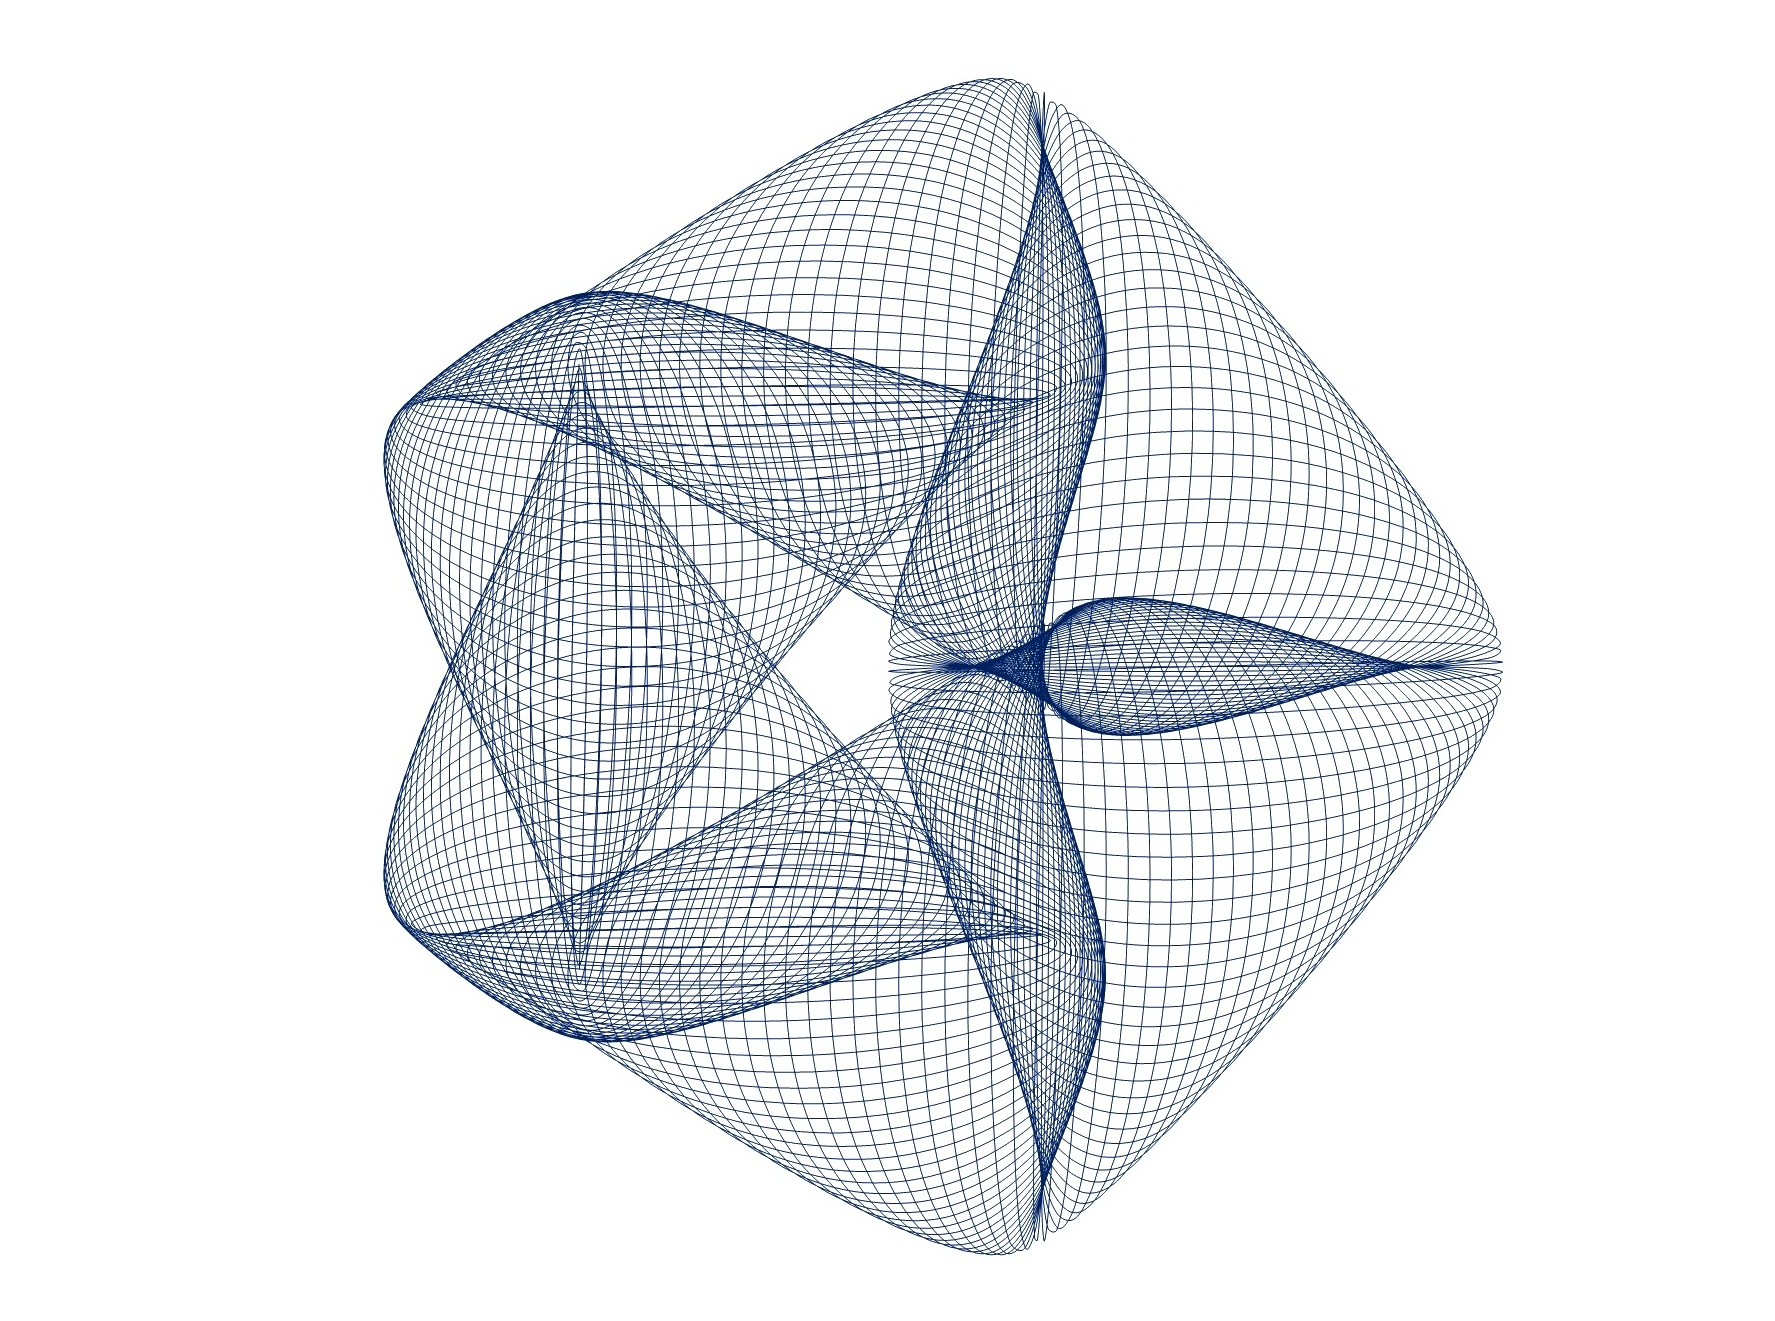
\includegraphics{../images/param_curve}}
    \end{figure}
\end{frame}

\begin{frame}
\frametitle{What is an arithmetic expression?}

Giving an arithmetic expression, we can parse it into a syntax tree. For example, the expression

\begin{equation}
(((((1 \times 2) \times 2) - 1) \times (2 + 1)) - 6)\label{eq:equation}
\end{equation}

and the parsed syntax tree

\begin{figure}[ht]
\centering
\resizebox{0.4\textheight}{!}{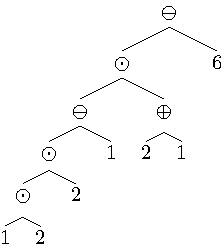
\includegraphics{../images/02-example-expression-syntax-tree.pdf}}
\caption{a tree representation of an arithmetic expression}\label{fig:syntaxtree}\label{fig:figure}
\end{figure}
\end{frame}

\begin{frame}
\frametitle{A definition of arithmetic expression}
\begin{definition}\label{def:arithmetic-expression}
    An arithmetic expression $a$ over $\mathbb{Q}$ is a structure given by the following production rules:
\begin{equation}\label{eq:productionrule}
\begin{aligned}
a &\longleftarrow x\\
a &\longleftarrow ( a + a )\\
a &\longleftarrow ( a - a )\\
a &\longleftarrow ( a \times a )\\
a &\longleftarrow ( a \div a )
\end{aligned}
\end{equation}
    where $x \in \mathbb{Q}$, and we denote this as $a \in \mathbb{E} \left [\mathbb{Q} \right ]$.
\end{definition}
\end{frame}

\begin{frame}
\frametitle{Evaluation of arithmetic expression}
We can define evaluation $\nu(a)$ of $a$ recursively as follows:
\begin{itemize}
  \item Constant leaf: for any $x \in \mathbb{Q}$, $\nu(x) = x$.
  \item Compositional node by $+$: For any $(a + b)$, $\nu((a + b)) = \nu(a) + \nu(b)$.
  \item Compositional node by $-$: For any $(a - b)$, $\nu((a - b)) = \nu(a) - \nu(b)$.
  \item Compositional node by $\times$: For any $(a \times b)$, $\nu((a \times b)) = \nu(a) \nu(b)$.
  \item Compositional node by $\div$: For any $(a \div b)$, if $\nu(b) \neq 0$, then $\nu((a \div b)) = \nu(a) / \nu(b)$.
\end{itemize}
Generally, the evaluation order of the arithmetic expression is not unique though the result is decided.
\end{frame}

\begin{frame}
    \frametitle{Threadlike expressions}
    Right-expanded and left-expanded threadlike expressions
    \begin{figure}[ht]
        \centering
        \resizebox{1.0\textheight}{!}{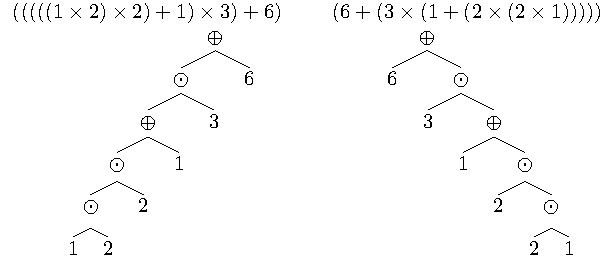
\includegraphics{../images/03-example-expression-syntax-tree-left-right.pdf}}
    \end{figure}
    The evaluation order of threadlike expressions is unique. We take left-expanded threadlike expressions as the standard form.
\end{frame}

\begin{frame}
    \frametitle{Case study}
    \begin{figure}[ht]\centering
    \resizebox{0.5\textwidth}{!}{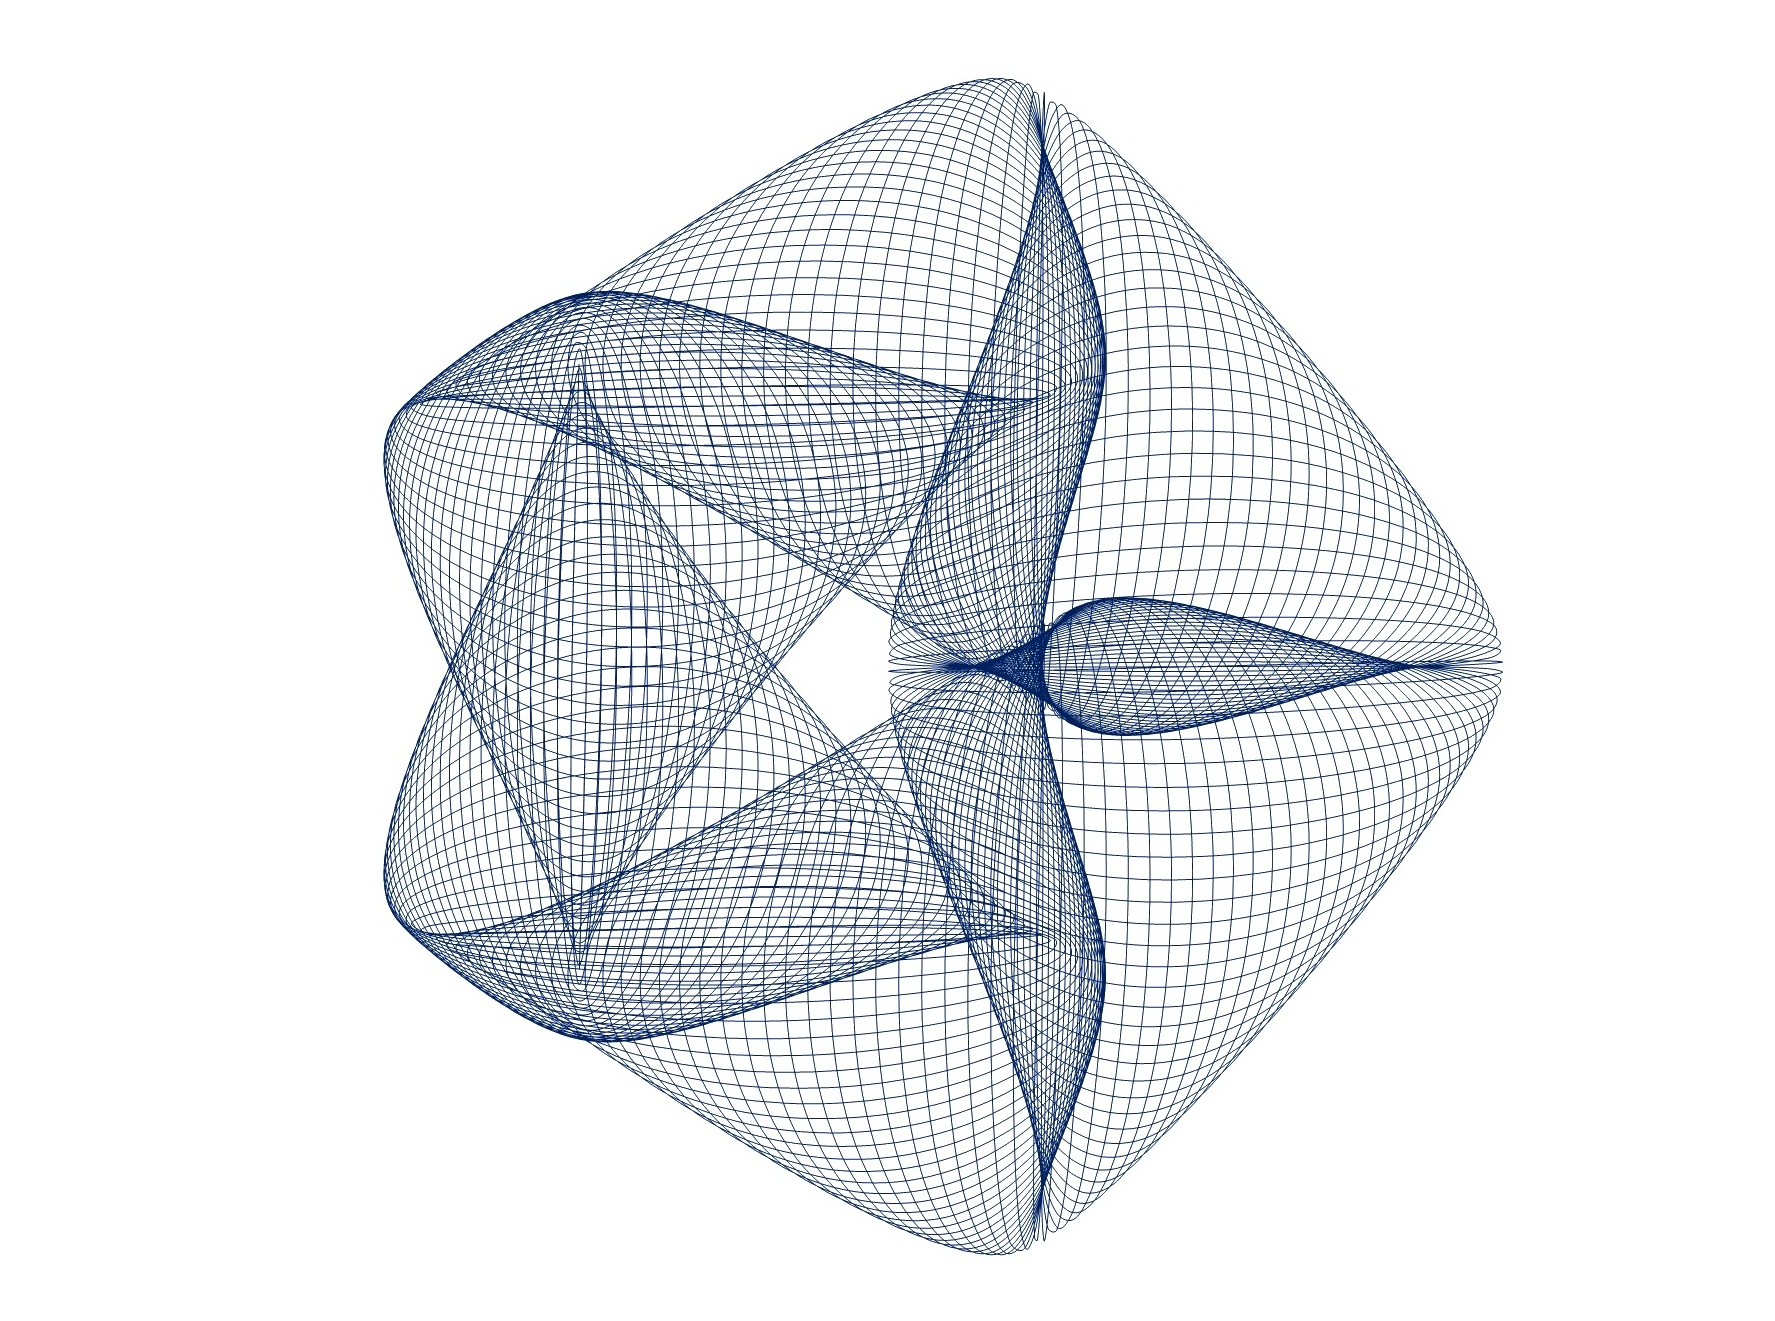
\includegraphics{../images/param_curve}}
    \end{figure}
\end{frame}

\begin{frame}
    \frametitle{Setting of $\mathfrak{E}_1$ space}
    The hyperbolic space equipped with the metric
    \[
        ds^2 = \frac{1}{y^2}(\frac{dx^2}{\mu^2} + \frac{dy^2}{\lambda^2})
    \]
    and a scalar field
    \[
        a = - \frac{x}{y}
    \]
    The flow equation is satisfied.
\end{frame}

\begin{frame}
    \frametitle{A grid on $\mathfrak{E}_1$ space}
    \begin{figure}[ht]\centering
    \resizebox{0.8\textwidth}{!}{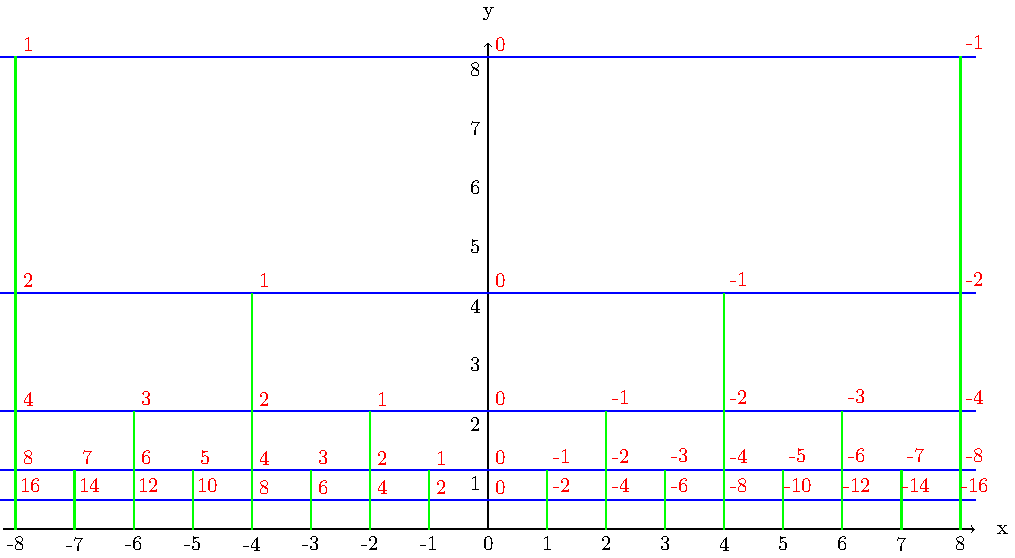
\includegraphics{../images/01-grid-example-1}}
    \end{figure}
\end{frame}

\begin{frame}
    \frametitle{Another grid on $\mathfrak{E}_1$ space}
    \begin{figure}[ht]\centering
    \resizebox{0.8\textwidth}{!}{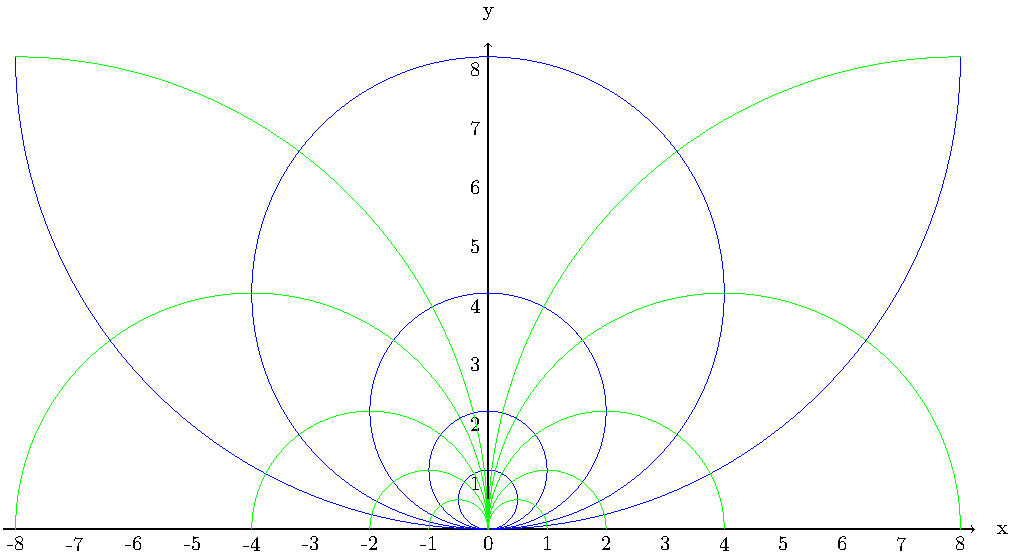
\includegraphics{../images/18-grid-example-2}}
    \end{figure}
\end{frame}

\begin{frame}
    \frametitle{Möbius transformation}
    \begin{columns}
        \begin{column}{0.5\textwidth}
            \begin{figure}[ht]\centering
            \resizebox{0.8\textwidth}{!}{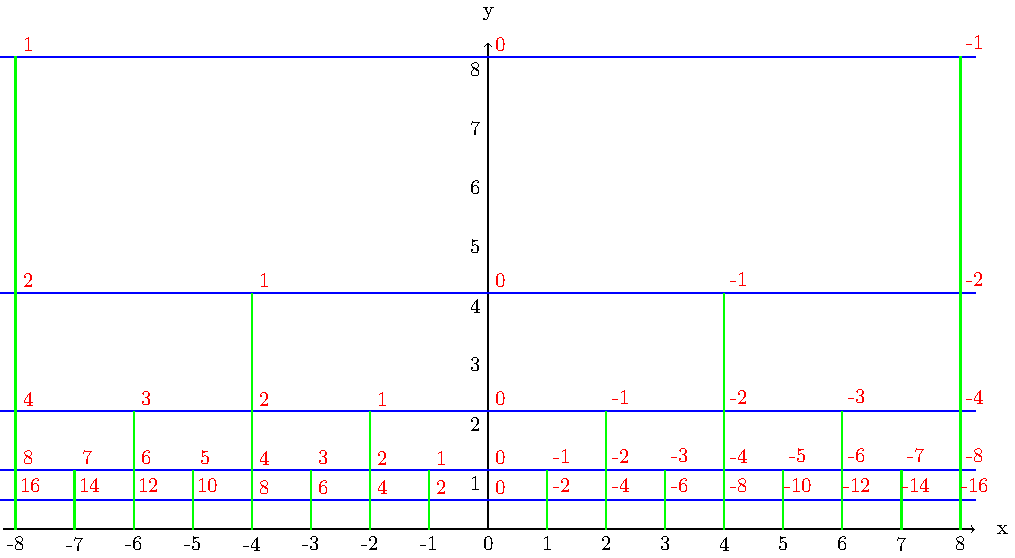
\includegraphics{../images/01-grid-example-1}}
            \end{figure}
        \end{column}
        \begin{column}{0.5\textwidth}
            \begin{figure}[ht]\centering
            \resizebox{0.8\textwidth}{!}{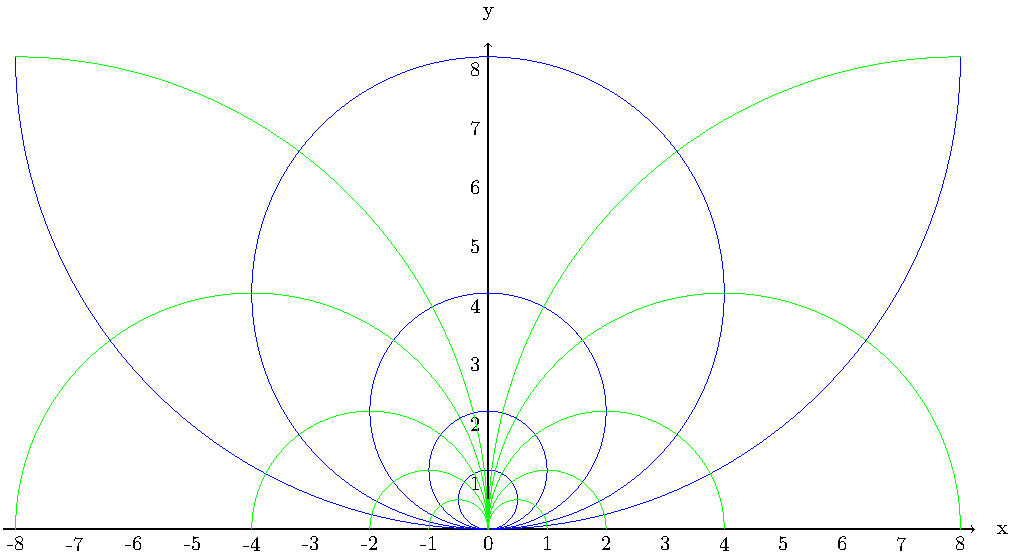
\includegraphics{../images/18-grid-example-2}}
            \end{figure}
        \end{column}
    \end{columns}
    \begin{center}
        \[
            z \mapsto - \frac{1}{z}
        \]
    \end{center}
\end{frame}

\begin{frame}
    \frametitle{Eigenfunction of the Laplacian}
    In our setting, \(A = \frac{1}{\mu y}\) and \(B = \frac{1}{\lambda y}\):

    \[
        \Delta f = y^2 \left(\mu^2 \frac{\partial^2 f}{\partial x^2} + \lambda^2 \frac{\partial^2 f}{\partial y^2}\right)
    \]

    And for the function \(f = - \frac{x}{y}\), we have

    \[
        \Delta f = - \frac{2 \lambda^2 x}{y} = 2 \lambda^2 f
    \]

    So, we reach the conclusion that the function \(f = - \frac{x}{y}\) is a eigenfunction of the Laplacian with eigenvalue \(2 \lambda^2\).
\end{frame}

\begin{frame}
    \frametitle{Two approaches towards arithmetic expression space?}
    We have several relevant structures:
    \begin{itemize}
        \item $E(F), (H, a), (Path, Integ)$
    \end{itemize}
    A constructive approach: from well-defined $E(Q)$, we introduce a proper topology and metric to form a space with
    a compatible condition
    \begin{enumerate}
        \item Convergence geometrically can lead to convergence of arithmetic evaluation
        \item The arithmetic evaluation can be extended to the whole topological space continuously
    \end{enumerate}
    An interpretative approach: we can interpret a special zigzag path of a well-defined space as an arithmetic
    expression.
    \begin{enumerate}
        \item Bijective: every threadlike arithmetic expression can be interpreted as a zigzag path, and versa vice
    \end{enumerate}
\end{frame}

\begin{frame}
    \frametitle{Unsolved problems}
    \begin{figure}[ht]\centering
    \resizebox{0.5\textwidth}{!}{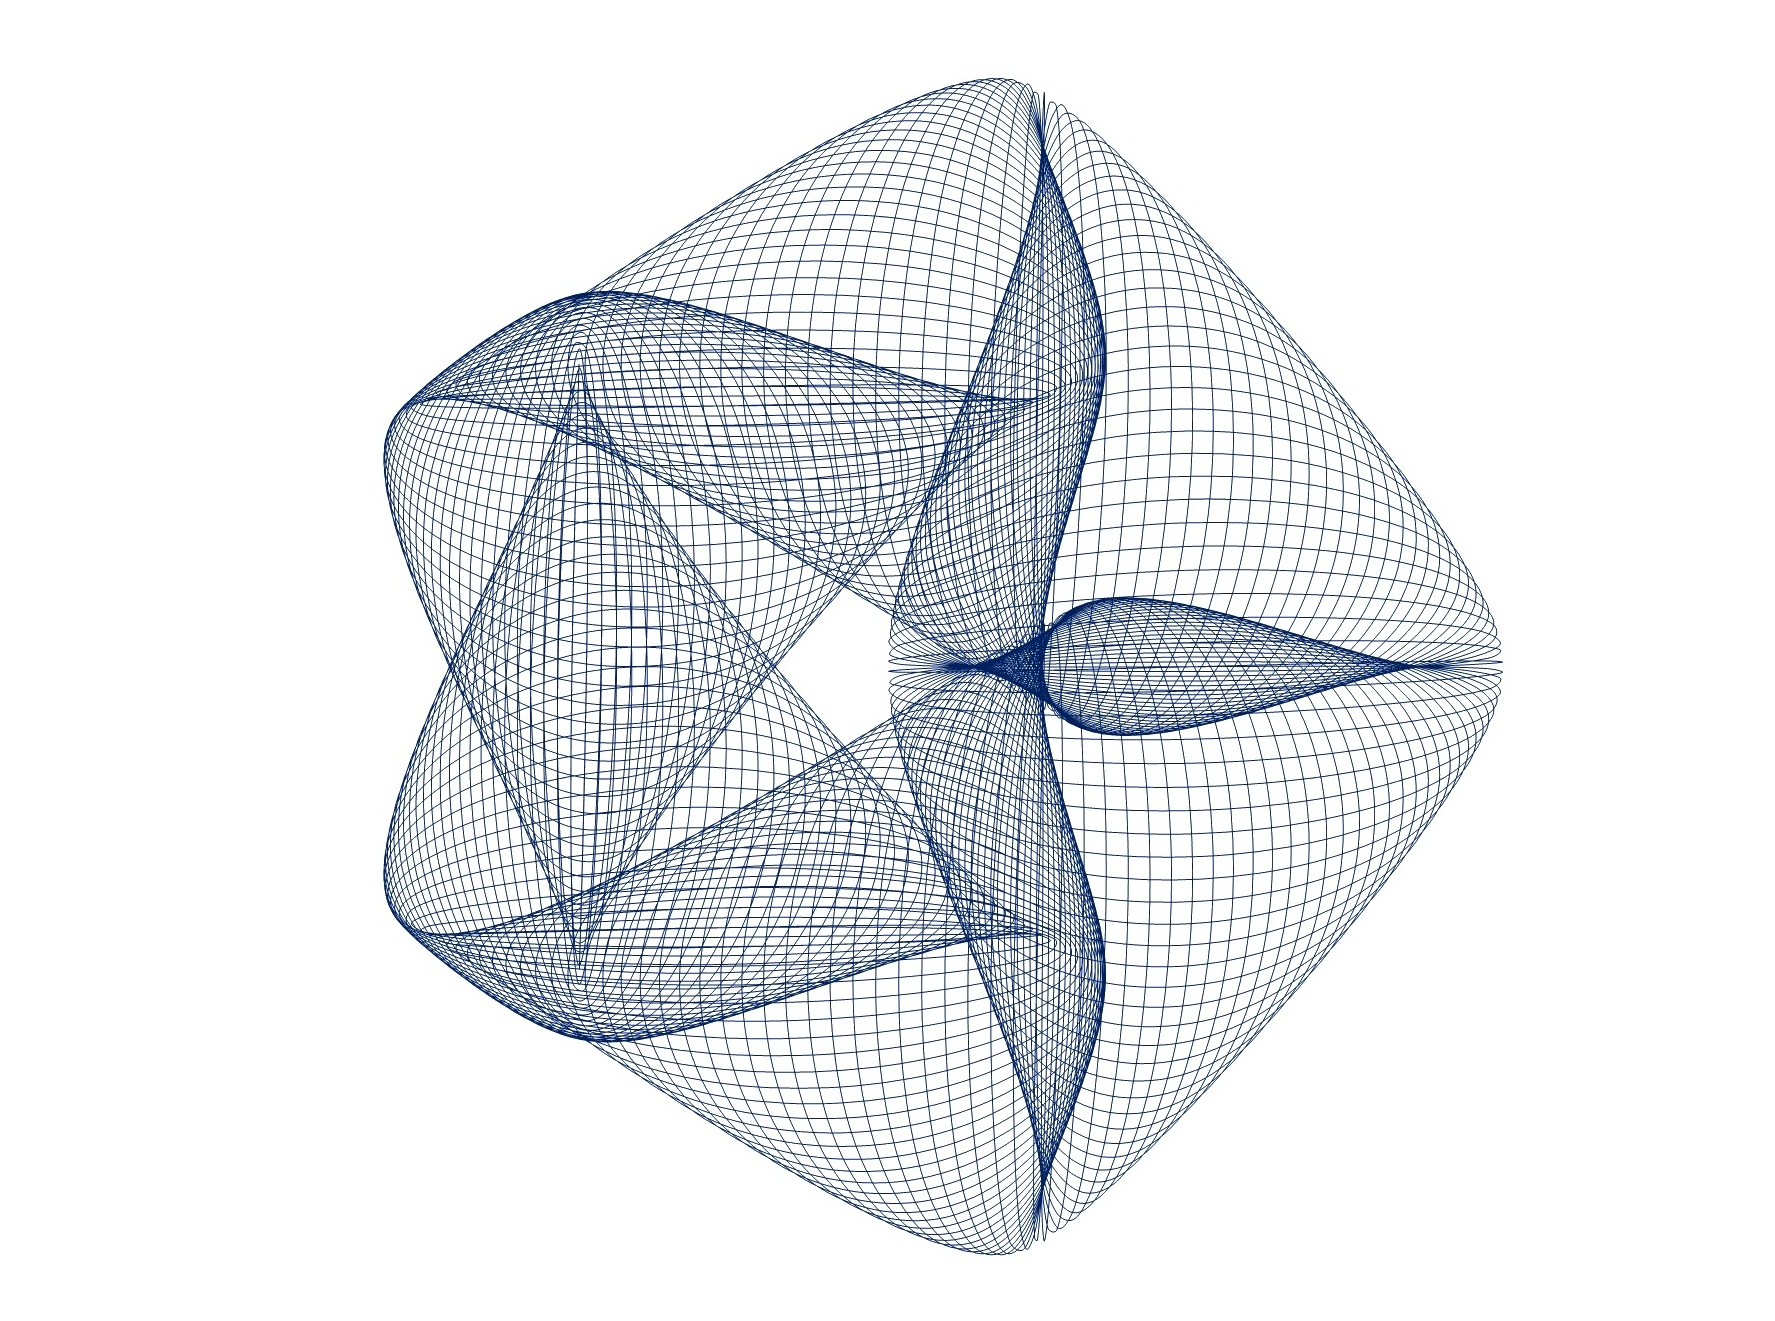
\includegraphics{../images/param_curve}}
    \end{figure}
\end{frame}

\begin{frame}
    \frametitle{More examples?}
    $\mathfrak{E_1}$ is too rigid, can we find a space that is more flexible?
    \begin{columns}
        \begin{column}{0.5\textwidth}
            \begin{figure}[ht]\centering
            \resizebox{0.8\textwidth}{!}{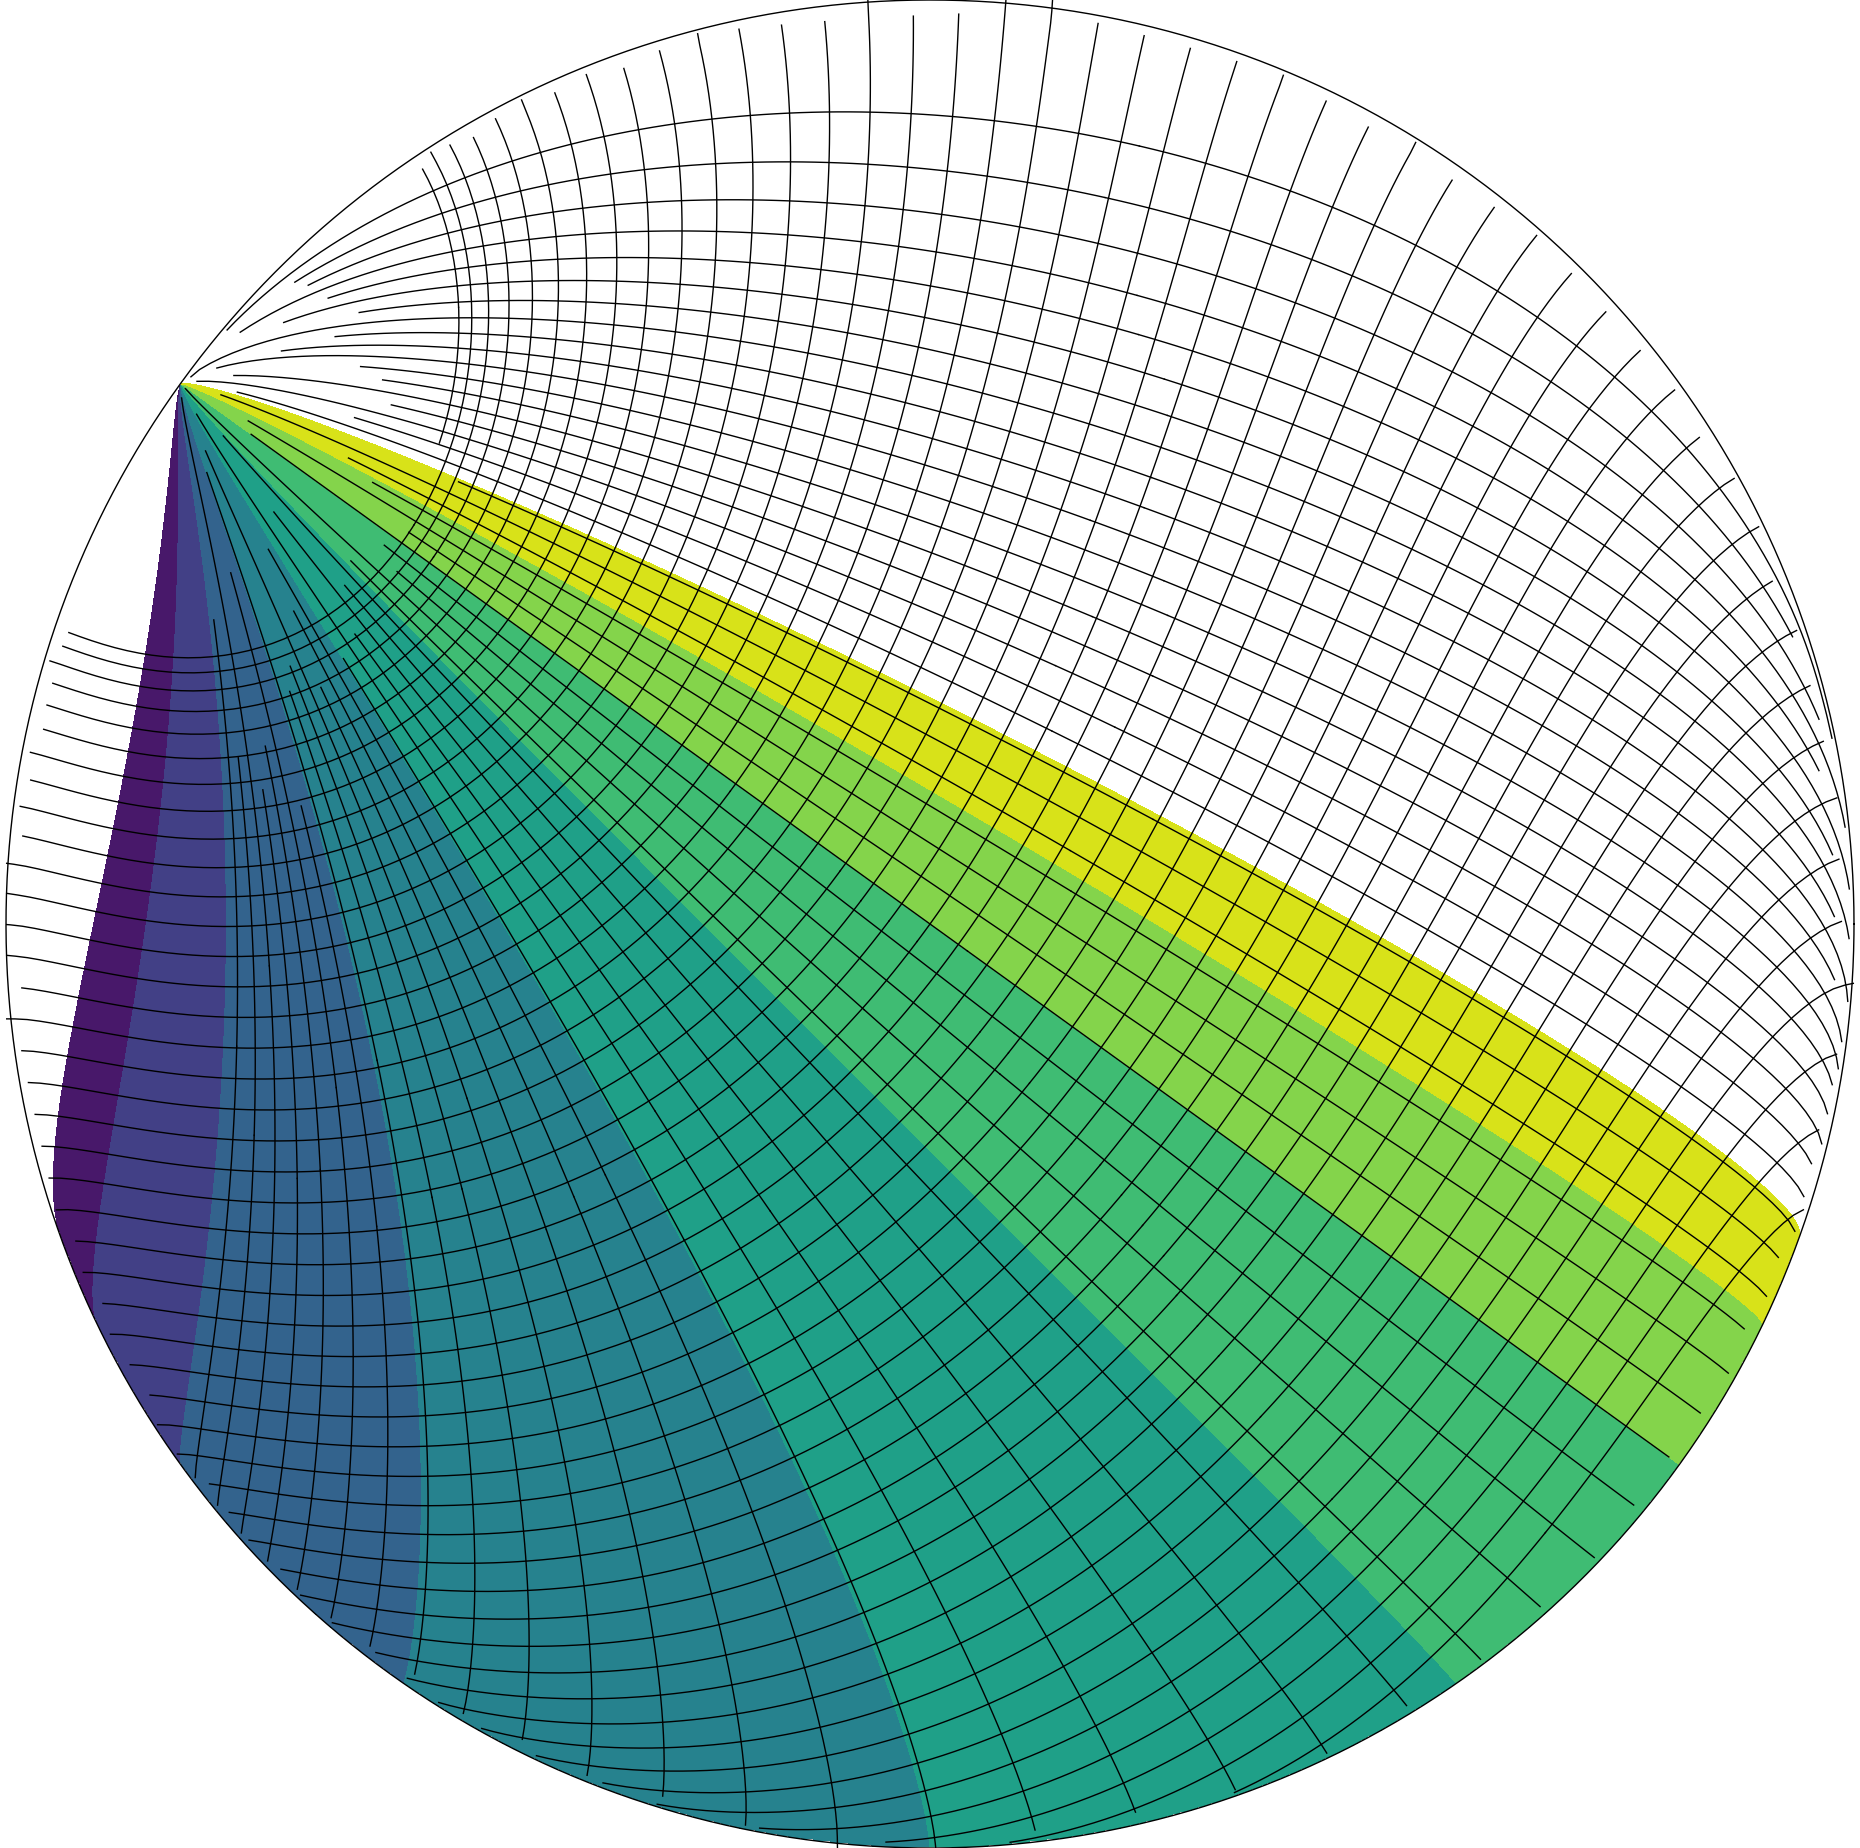
\includegraphics{../images/e2_grid_cg}}
            \end{figure}
        \end{column}
        \begin{column}{0.5\textwidth}
            \begin{figure}[ht]\centering
            \resizebox{0.8\textwidth}{!}{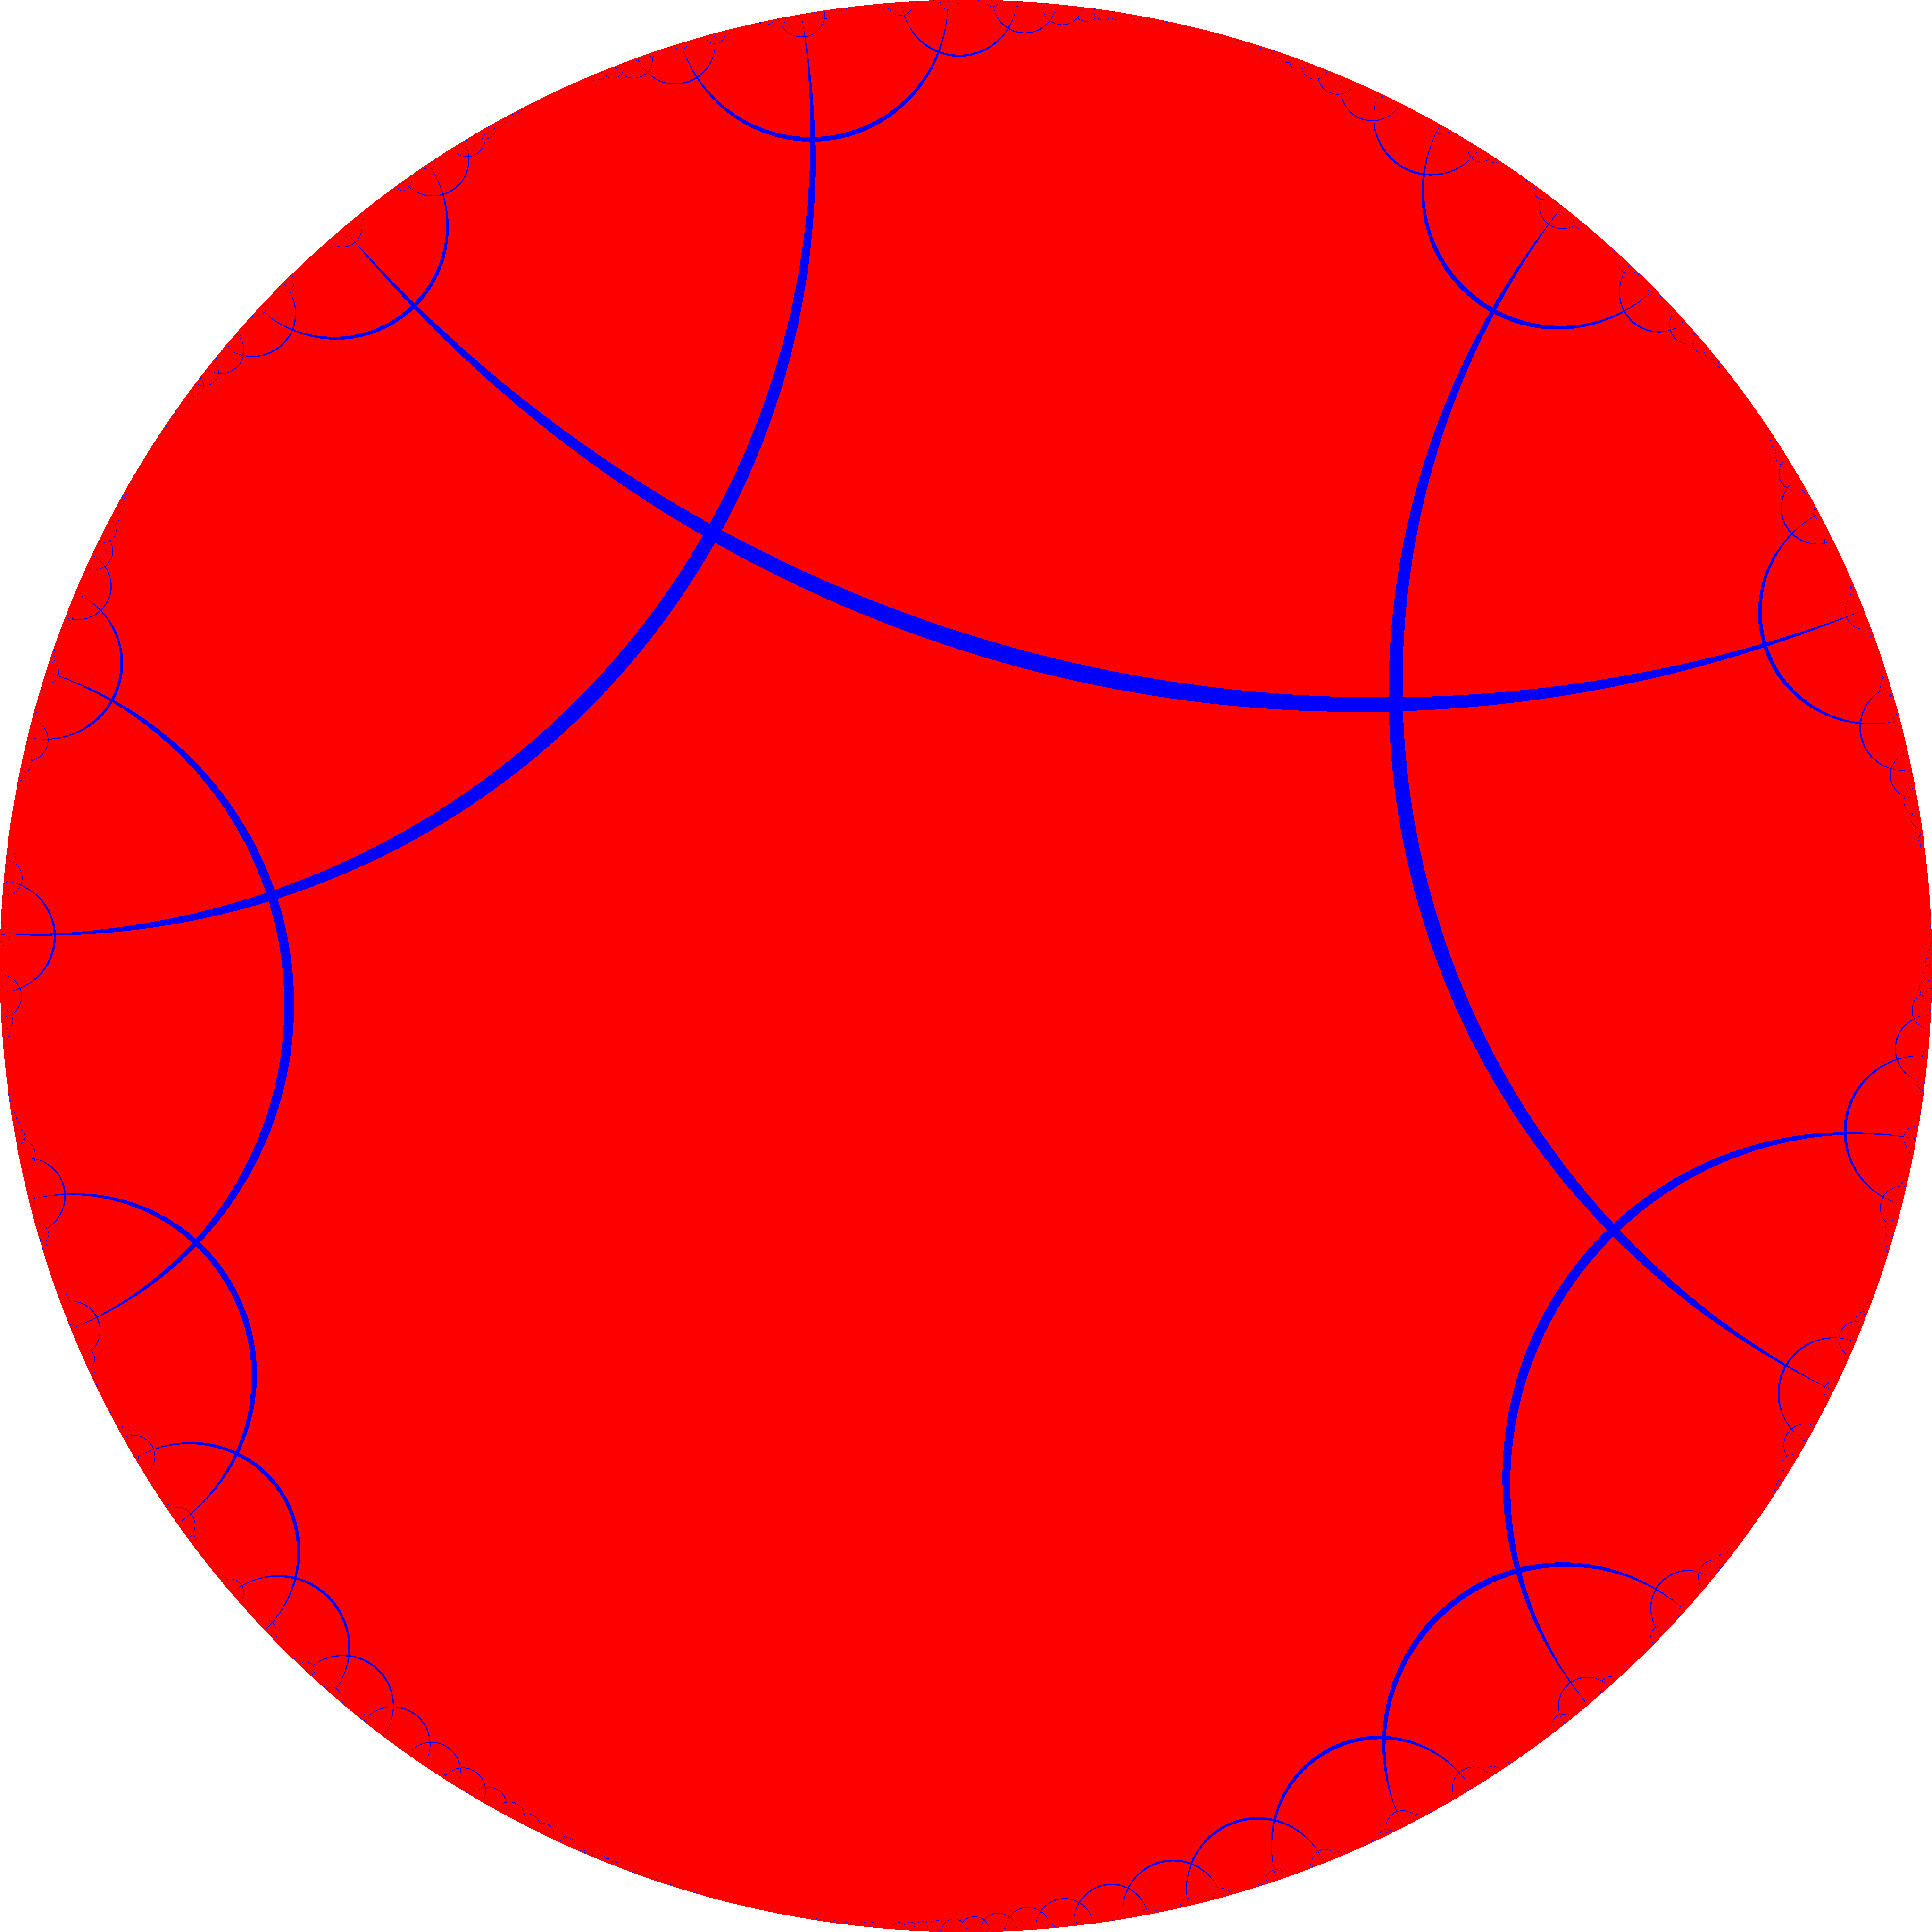
\includegraphics{../images/t4096}}
            \end{figure}
        \end{column}
    \end{columns}

\end{frame}

\begin{frame}
    \frametitle{Existence theorems}
    \begin{itemize}
        \item Local metric existence theorem
        \item Proper assignment existence?
    \end{itemize}
\end{frame}

\begin{frame}
    \frametitle{Global structure and classification}

    \emph{Local structure}: totally decided by the flow equation.

    \emph{Classification of the global structure}

\end{frame}

\begin{frame}
\frametitle{Eigenfunction of Laplacian}
    Eigenfunction of Laplacian in $\mathfrak{E_1}$ space might not be a special case.
\end{frame}

\begin{frame}
    \frametitle{AEG over complex numbers}
    We cannot make $\times -1$ compatible with the flow equation in the real number case,
    but we can do it in the complex number case easily with the imaginary unit $i$.
    complex arithmetic expression space is mandatory in the theory.
\end{frame}

\begin{frame}
    \frametitle{Hyper-operations}
    Repeating one operation to generate operation in next order
    \begin{table}[!ht]
        \centering
        \begin{tabular}{|l|l|l|}
            \hline
            Order & Operation &  Notion \\
            \hline
            0 & Succession & $a + 1$ \\
            1 & Addition & $a + b$ \\
            2 & Multiplication & $a \times b$ \\
            3 & Exponentiation & $a^b$ \\
            4 & Tetration & $a [4] b$ \\
            5 & Pentation & $a [5] b$ \\
            6 & Hexation & $a [6] b$ \\
            \hline
       \end{tabular}\label{tab:table}
    \end{table}
    Can we compose high dimensional AEG space by hyper-operations?
\end{frame}

\section{Complex analysis in a nutshell}

\begin{frame}
    \frametitle{Complex analysis in a nutshell}
    \begin{enumerate}
        \item Complex differentiable
        \item Analytic
        \item Holomorphic
        \item Conformal
        \item Maximum modulus principle
    \end{enumerate}
\end{frame}

\begin{frame}
    \frametitle{Complex differentiable}
    The Cauchy-Riemann condition
    \[
        \frac{\partial u}{\partial x} = \frac{\partial v}{\partial y}, \quad \frac{\partial u}{\partial y} = - \frac{\partial v}{\partial x}
    \]
    setup the compatibility between the complex structure and the differential structure, which means any path approaching
    a point should lead to the same derivative.
    \[
        \frac{\delta f}{\delta z} = \frac{\delta u + i \delta v}{\delta x + i \delta y}
    \]
    \[
        \left. \frac{\delta f}{\delta z} \right \rvert_{\delta y=0}= \frac{\delta u}{\delta x} + i \frac{\delta v}{\delta x}
    \]
    \[
        \left. \frac{\delta f}{\delta z} \right \rvert_{\delta x=0} = - i \frac{\delta u}{\delta y} + \frac{\delta v}{\delta y}
    \]
\end{frame}

\begin{frame}
    \frametitle{Holomorphic function}
    A function is holomorphic if it is complex differentiable at every point in its domain.
    \[
        f(z) = u(x, y) + i v(x, y)
    \]
    $u$ and $v$ are a pair of harmonic functions, which satisfy the Laplace equation, and are conjugate to each other.
\end{frame}

\begin{frame}
    \frametitle{Analytic function}
    A function is analytic if and only if its Taylor series at point $z_0$ converges to the function in some neighborhood of $z_0$
    for every $z_0$ in its domain.
    \[
        f(z) = \sum_{n=0}^\infty a_{n} \left( z-z_0 \right)^{n} = a_0 + a_1 (z-z_0) + a_2 (z-z_0)^2 + \cdots
    \]
\end{frame}

\begin{frame}
    \frametitle{Cauchy integral formula}
    A function $f$ is holomorphic in a domain and continuous on the boundary of the domain.
    For any point $z$ in the domain, $C$ is a closed rectifiable curve which has winding number one around $z$,
    and $C$ is contained in the domain, then we have
    \[
        f(z) = \frac{1}{2 \pi i} \oint_{C} \frac{f(\zeta)}{\zeta - z} d\zeta
    \]
    We can use boundary value to determine the value of the function in the domain.
\end{frame}

\begin{frame}
    \frametitle{Conformal mapping}
    \begin{figure}[ht]\centering
    \resizebox{0.6\textwidth}{!}{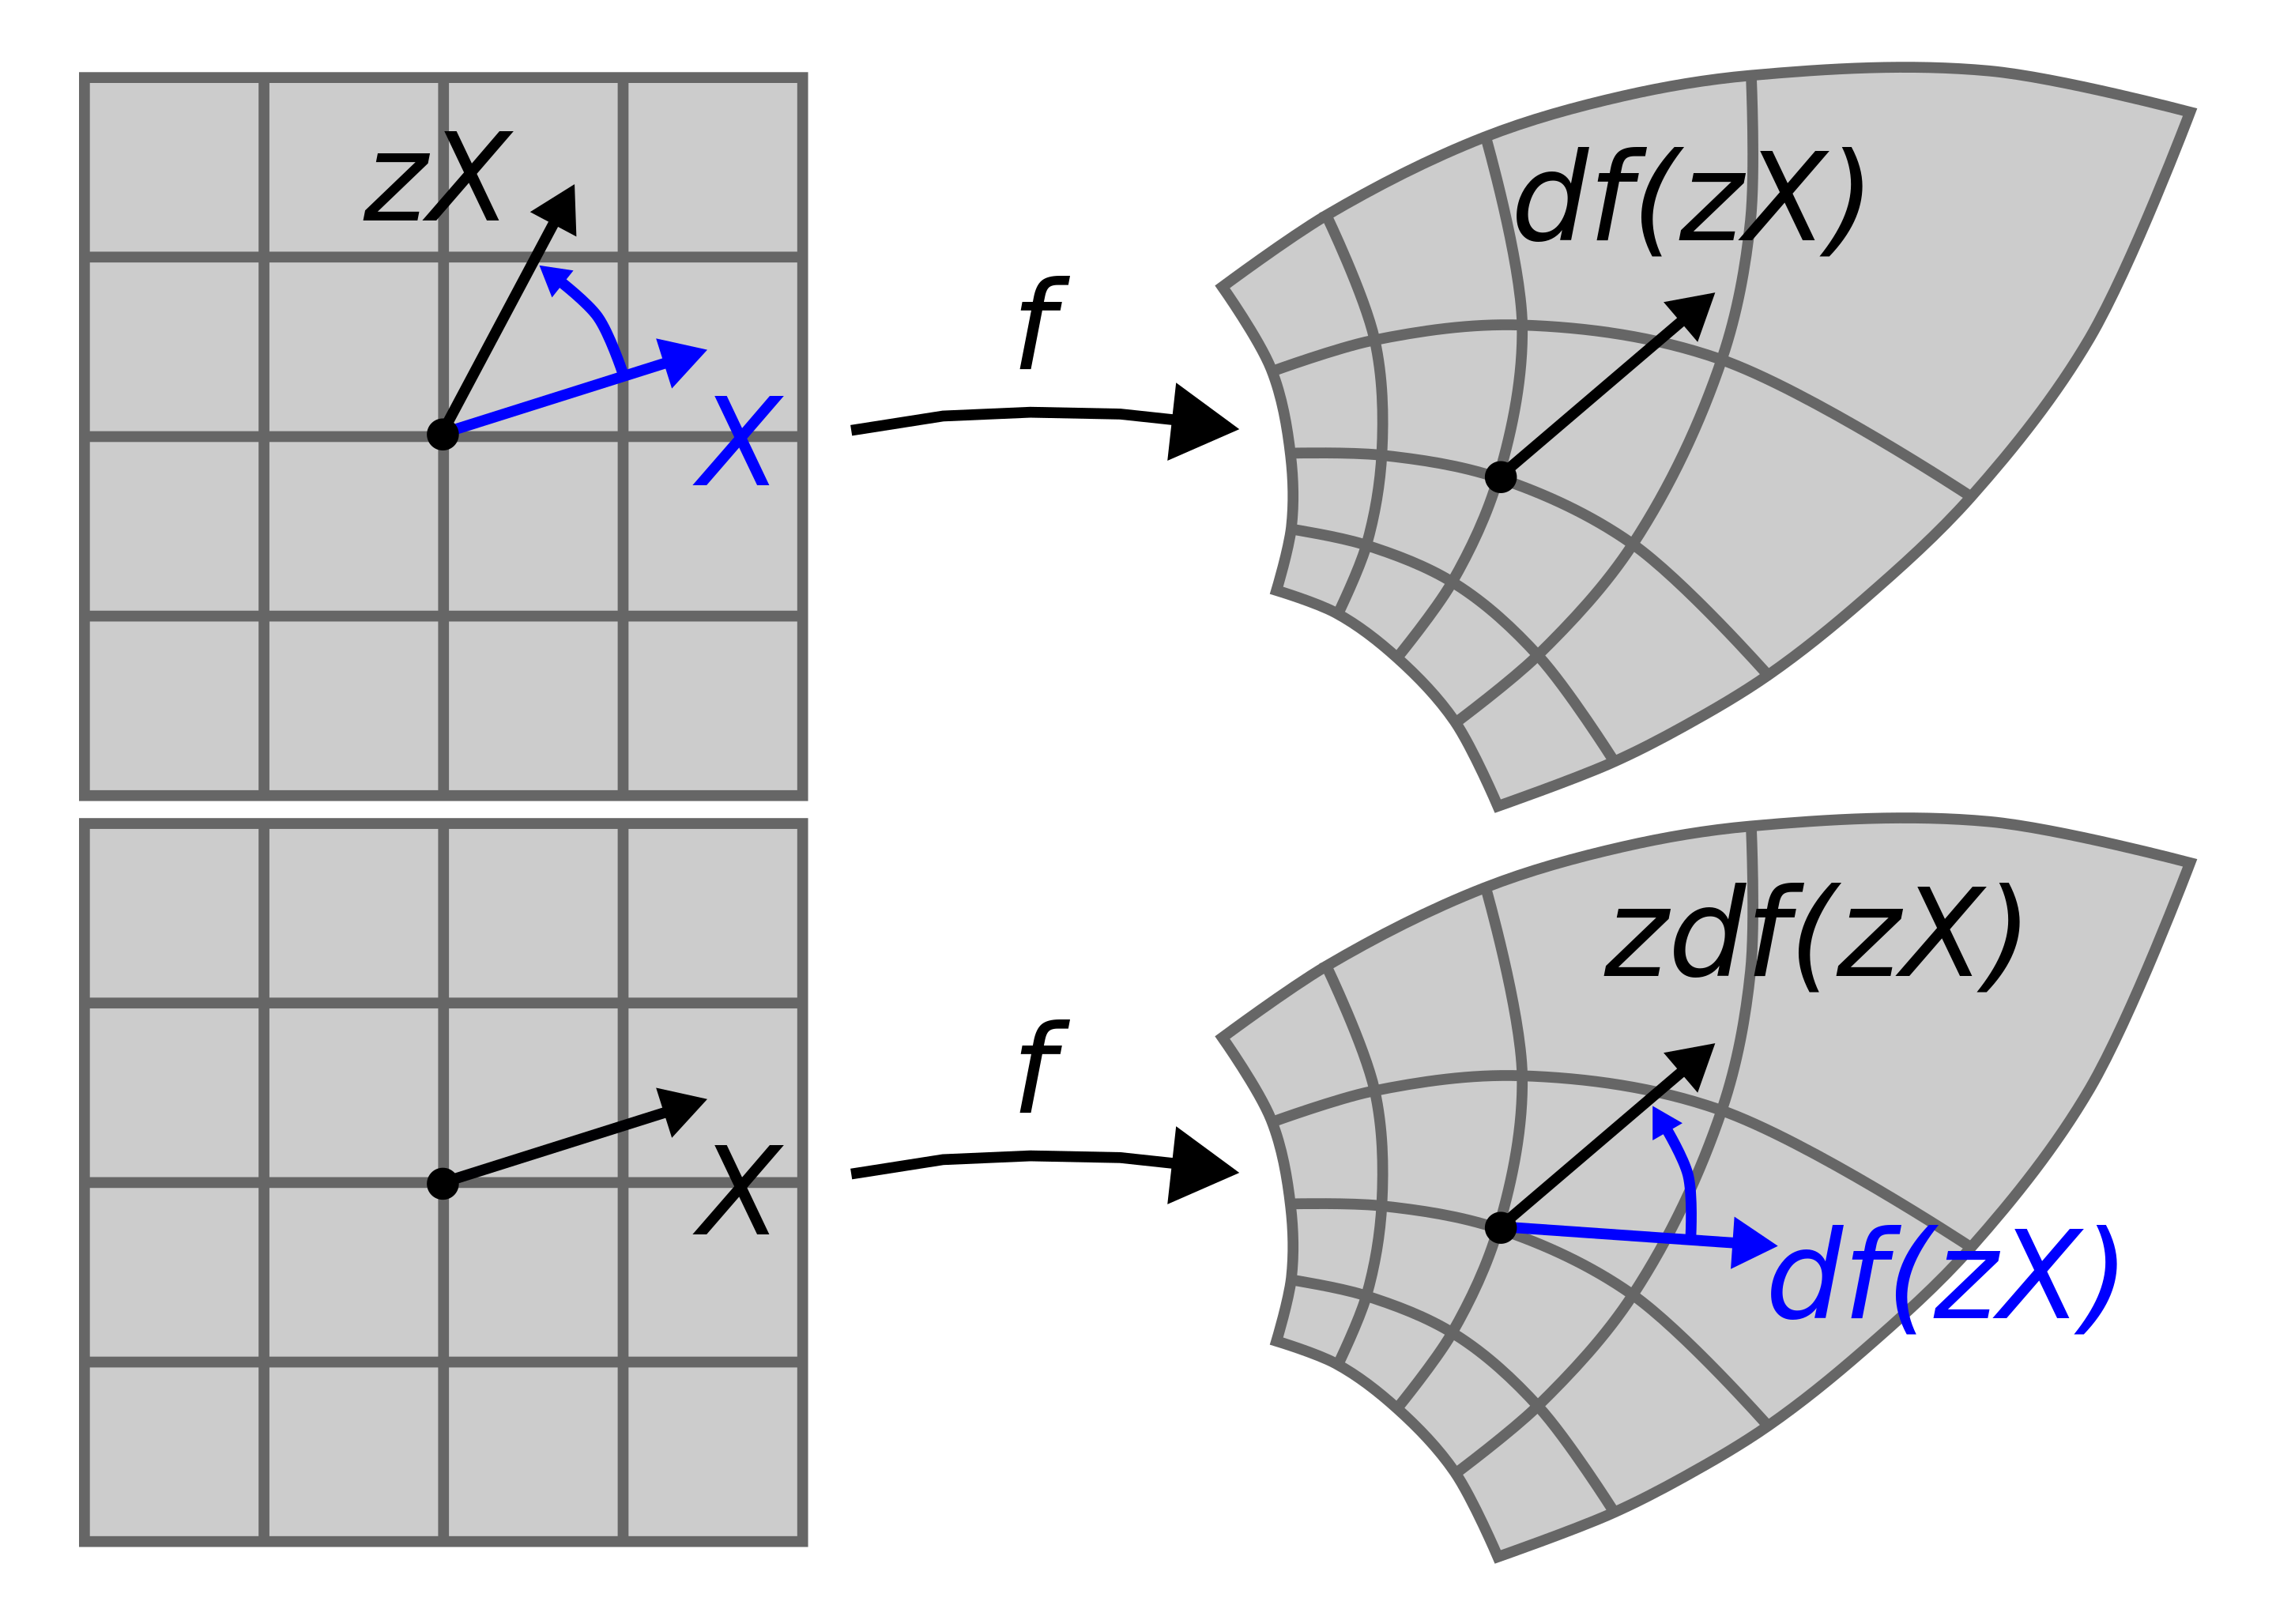
\includegraphics{../images/conformal}}
    \end{figure}
    \small{image credit: https://en.wikipedia.org/wiki/Cauchy-Riemann\_equations}
\end{frame}

\begin{frame}
    \frametitle{Maximum modulus principle}
    The modulus of a holomorphic function cannot exhibit a strict maximum that is strictly within its domain.
    \begin{figure}[ht]\centering
    \resizebox{0.3\textwidth}{!}{
\includegraphics{../images/maximum_modulus_principle}}
    \end{figure}
    \small{image credit: https://en.wikipedia.org/wiki/Maximum\_modulus\_principle}
\end{frame}

\section{Future directions: geometry, analysis and computation}

\begin{frame}
    \frametitle{Future directions: geometry, analysis and computation}
    \begin{enumerate}
        \item Geometry
        \item Analysis
        \item Computation
    \end{enumerate}
\end{frame}

\begin{frame}
    \frametitle{Geometry}
    \begin{figure}[ht]\centering
    \resizebox{0.5\textwidth}{!}{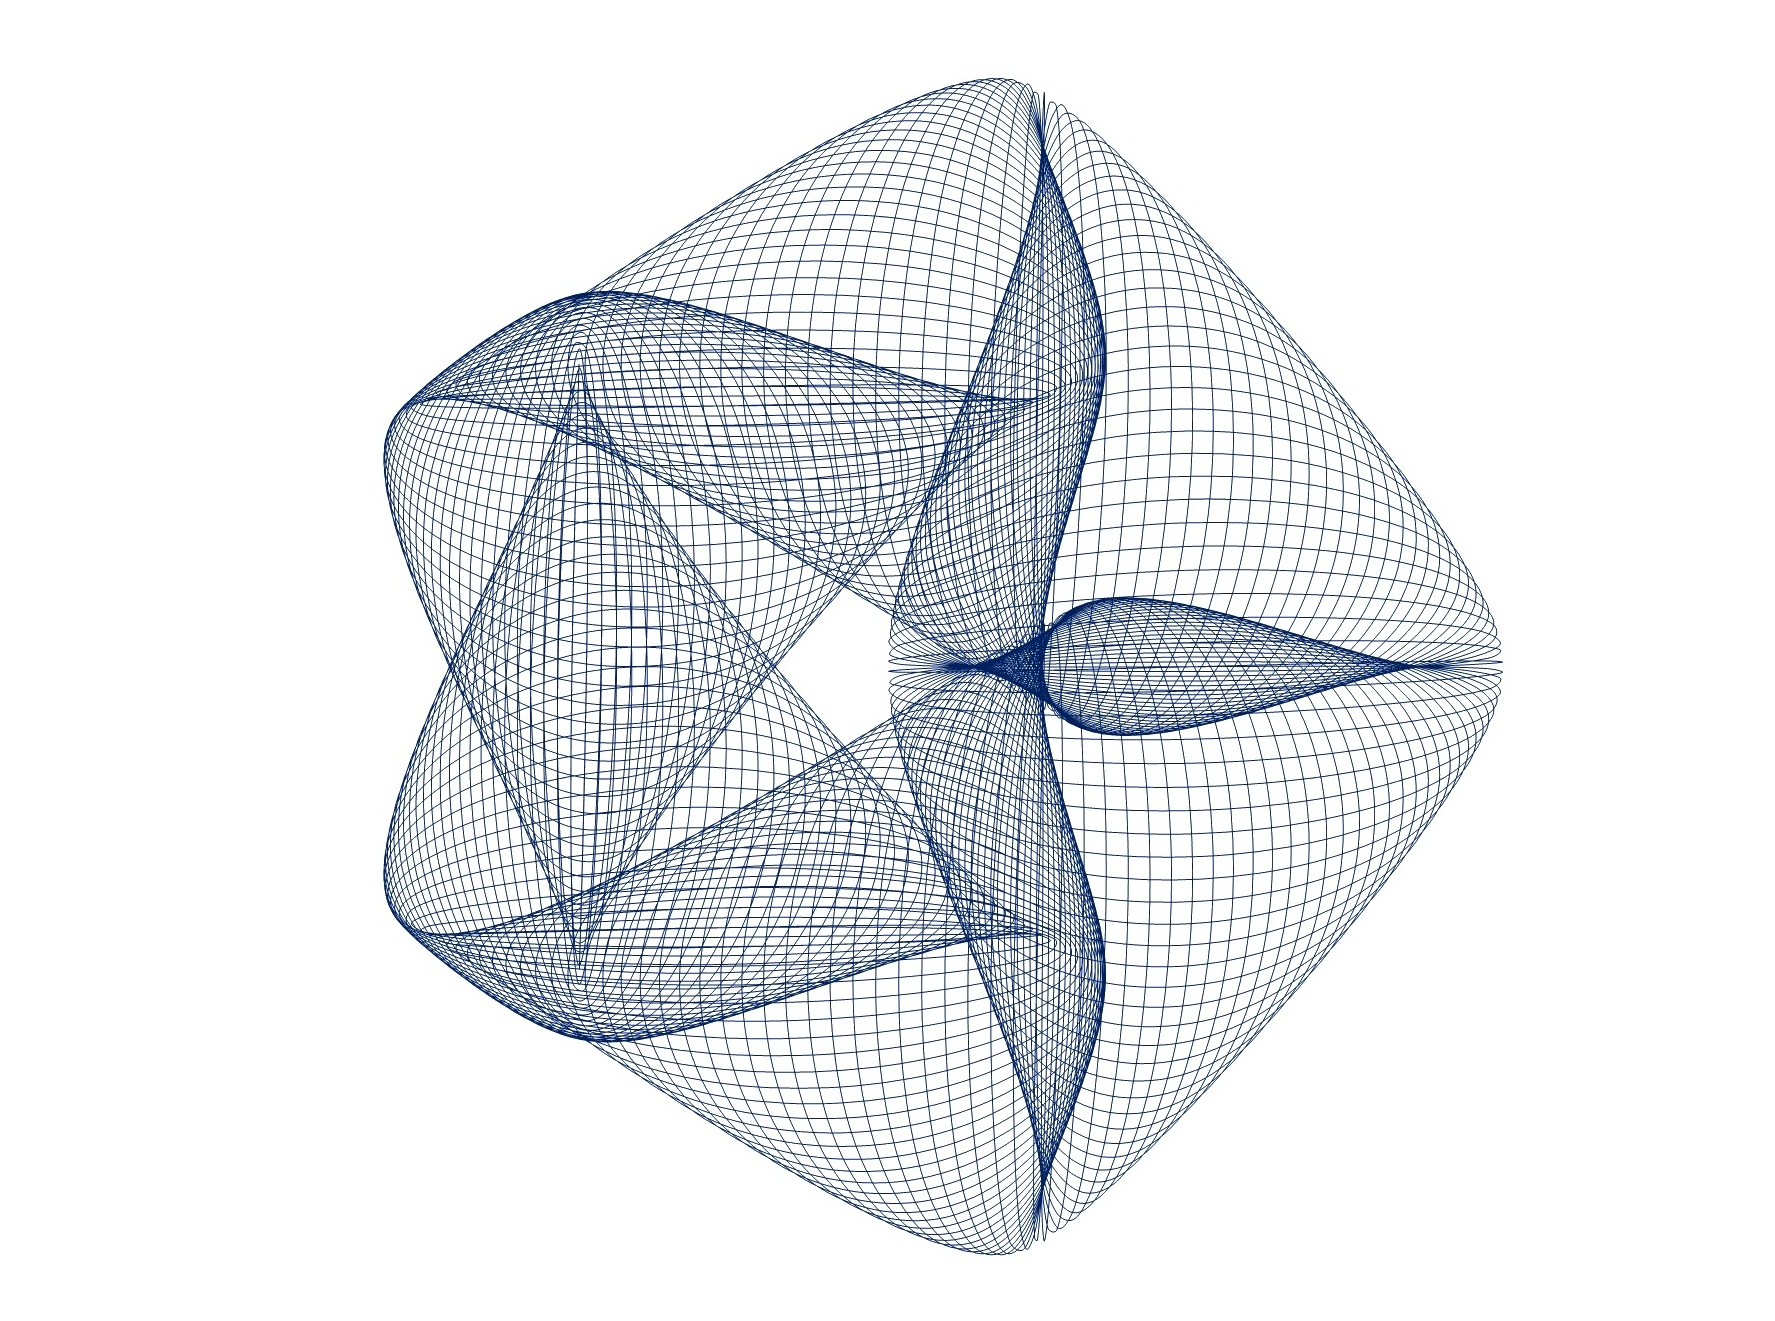
\includegraphics{../images/param_curve}}
    \end{figure}
\end{frame}

\begin{frame}
    \frametitle{Arithmetic torsion at scale}
    \begin{columns}
        \begin{column}{0.5\textwidth}
            We scale up the step size

            For one step, we have
            \begin{equation}
            (x + 1) \times 2 - (x \times 2 + 1) = 1
            \end{equation}

            Extending this to two steps, we encounter a different situation:
            \begin{equation}
            (x + 2) \times 4 - (x \times 4 + 2) = 6
            \end{equation}

            And for three steps, the pattern continues:
            \begin{equation}
            (x + 3) \times 8 - (x \times 8 + 3) = 21
            \end{equation}
        \end{column}
        \begin{column}{0.5\textwidth}
            \begin{center}
                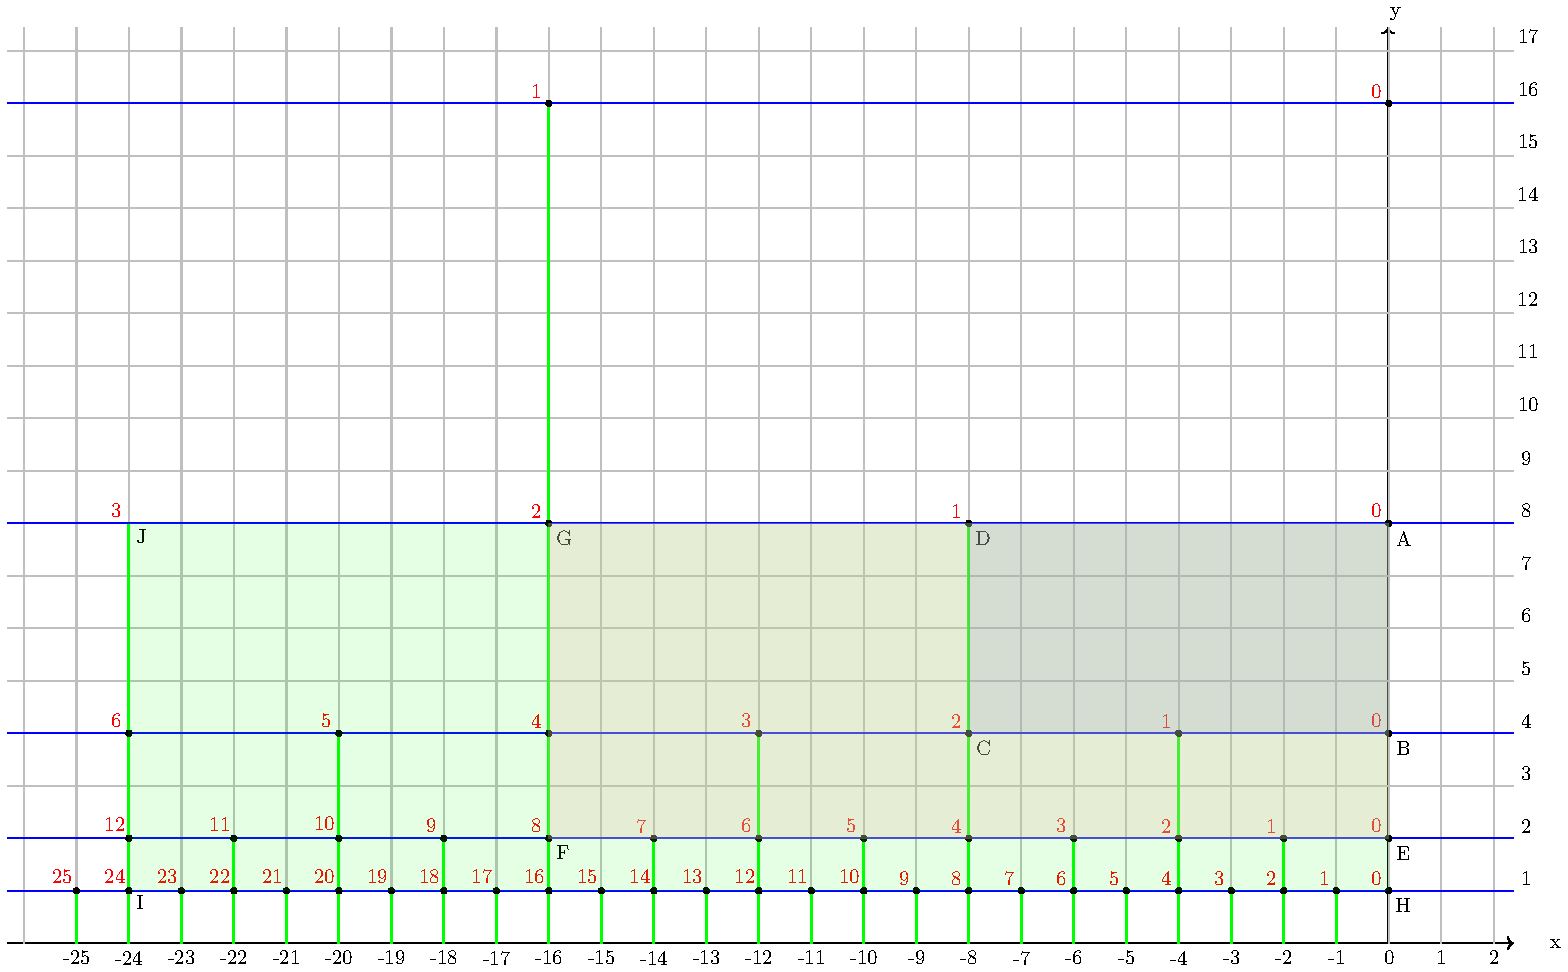
\includegraphics[width=1.0\textwidth]{../images/17-area-formula}
            \end{center}
        \end{column}
    \end{columns}
\end{frame}

\begin{frame}
    \frametitle{Area formula}
    \[
        d\tau = (a_0 + \mu du) e^{\lambda dv} - (a_0 e^{\lambda dv} + \mu du)
    \]

    \[
        d\tau = \mu \lambda du dv
    \]

    and because
    \[
        dS = \sqrt{A^2B^2 - F^2} du dv
    \]

    \begin{equation}
        \frac{d\tau}{\mu \lambda} = \frac{dS}{\sqrt{A^2B^2 - F^2}}
    \end{equation}
\end{frame}

\begin{frame}
    \frametitle{Curvature?}
    Arithmetic torsion is a quantity defined as a measure to reflect how the generators are non-commutative.
    It is defined on path, but when we scale up the step size, we find that torsion is
    related to the size of an area.

    Similar case can be found in the curvature of a surface, stated by the Gauss-Bonnet theorem.

    Can we find a connection between arithmetic torsion and curvature?
\end{frame}

\begin{frame}
    \frametitle{A broken clue?}
    \begin{center}
        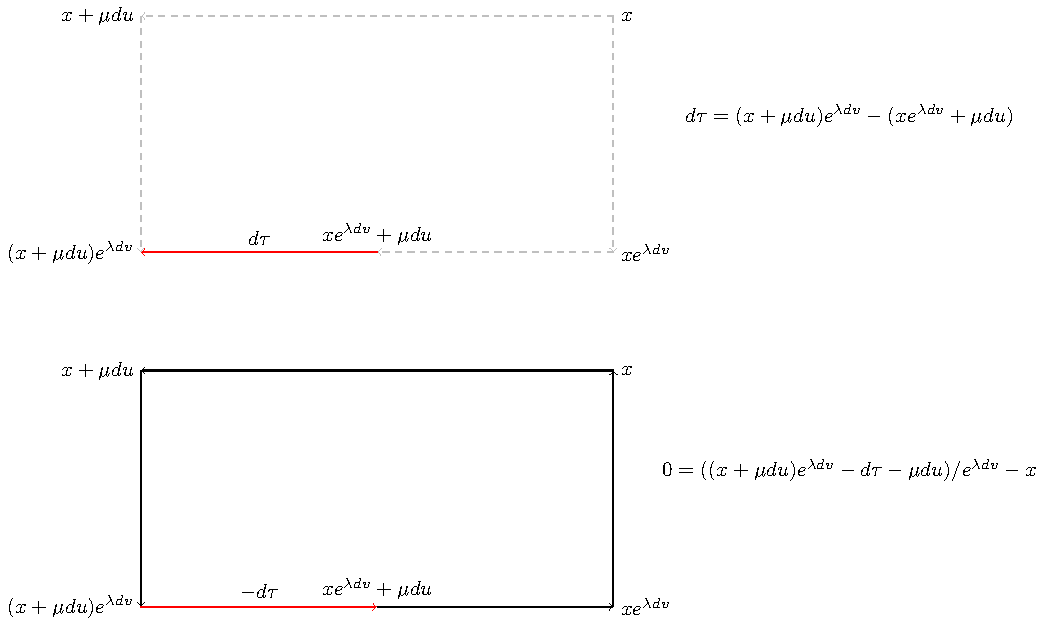
\includegraphics[width=0.7\textwidth]{../images/19-curl}
    \end{center}
\end{frame}

\begin{frame}
    \frametitle{Analysis}
    \begin{figure}[ht]\centering
    \resizebox{0.5\textwidth}{!}{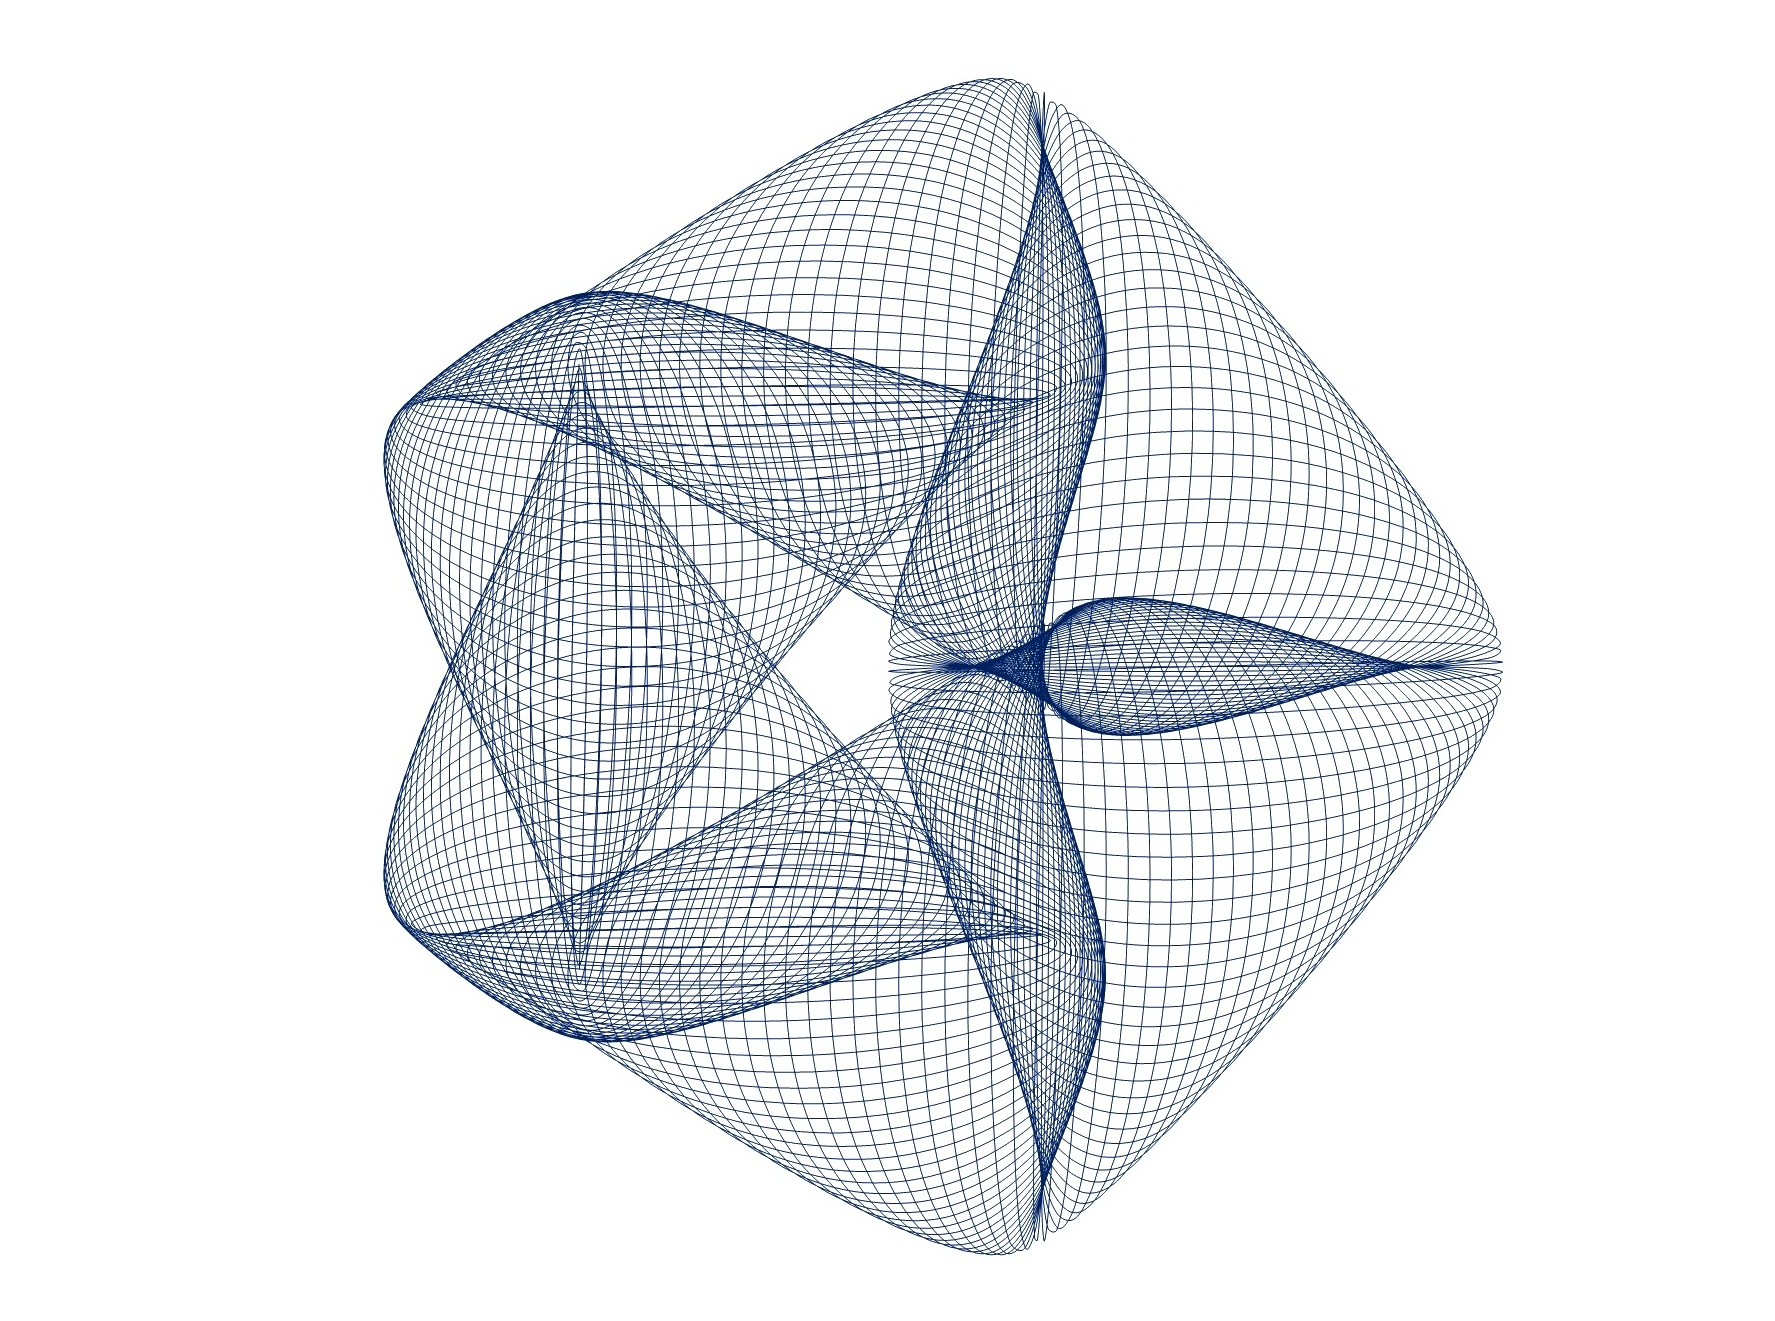
\includegraphics{../images/param_curve}}
    \end{figure}
\end{frame}

\begin{frame}
    \frametitle{Path integration?}
    We may extends Riemann integral to a path integral.
    What properties should the path integral have? Is the eigenfunction of Laplacian in $\mathfrak{E}_1$ a special case?
\end{frame}

\begin{frame}
    \frametitle{Flow equation and Cauchy–Riemann equations?}
    The picture of flow equation
    \[
        \frac{da}{ds} = \mu \cos \theta + a \lambda \sin \theta
    \]
    is that any path escape from a point leads to a different value.
    If we reverse the direction of the path, we have another interpretation of the flow equation.
    It can be also interpreted as a differentiability condition, any path approaching a point should lead to the same
    derivative, which is similar to the Cauchy–Riemann equations in complex analysis.
\end{frame}

\begin{frame}
    \frametitle{Maximum value principle?}
    For any $a$, we have a $\theta$ make $\frac{da}{ds}$ positive
    \[
        \frac{da}{ds} = \mu \cos \theta + a \lambda \sin \theta
    \]
    This means a maximum value principle is satisfied,
    which is similar to the maximum modulus principle in complex analysis.
\end{frame}

\begin{frame}
    \frametitle{Eigenfunction of Laplacian}
    In $\mathfrak{E_1}$ space, assignment $a$ is eigenfunction of Laplacian with eigenvalue $2 \lambda^2$.
    When $\lambda = 0$, it is pure additive case, and the curvature is zero also, and $a$ is harmonic.
\end{frame}

\begin{frame}
    \frametitle{Other analysis theories?}
    Formulate our systems as a tuple of
    \begin{itemize}
        \item $E(F), (H, a), (Path, Integ)$
    \end{itemize}
    Here we have
    \begin{itemize}
        \item $E(F)$: Expressions over a field $F$
        \item $(H, a)$: A scalar field "assignment" $a$ on a space $H$
        \item $(Path, Integ)$: all paths can be interpreted as an integral
    \end{itemize}
    Can we find more examples? Does complex analysis belong to this structure?
    We conjecture that complex analysis is a 1-dimensional additive AEG theory.
\end{frame}

\begin{frame}
    \frametitle{Tube structure?}
    \begin{figure}[ht]\centering
    \resizebox{0.8\textwidth}{!}{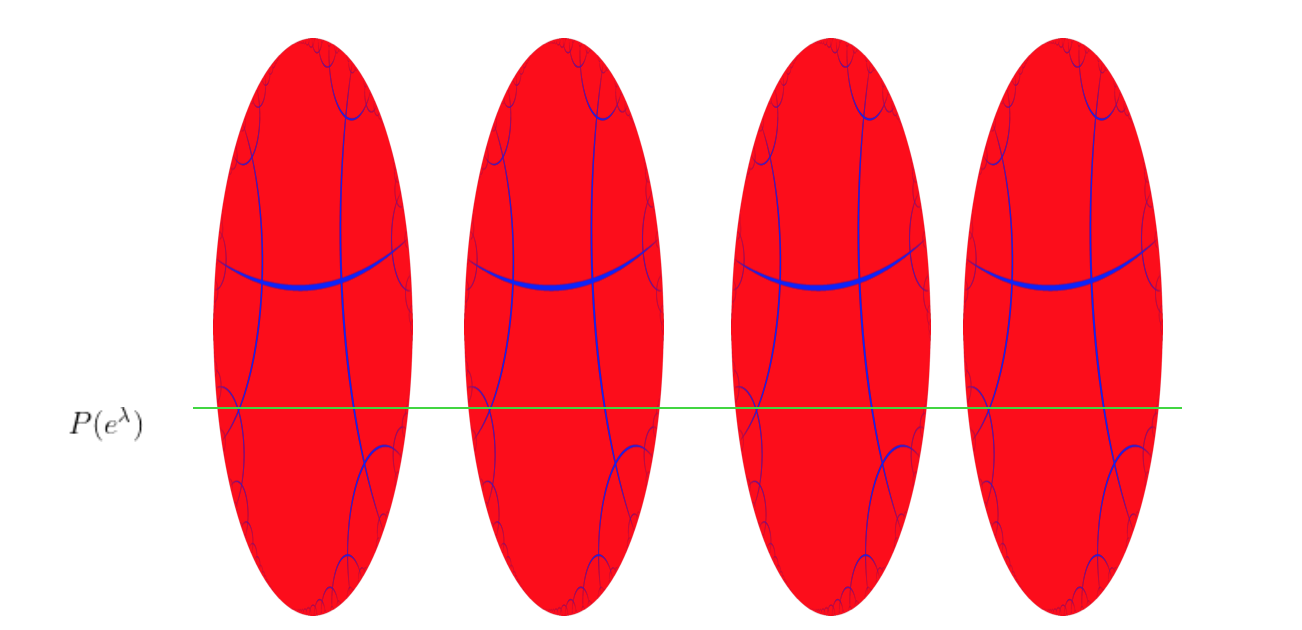
\includegraphics{../images/tube}}
    \end{figure}
    Real version and complex version.
    A polynomial as a fiber across the AEG spaces with different generators.
\end{frame}

\begin{frame}
    \frametitle{Computation}
    \begin{figure}[ht]\centering
    \resizebox{0.5\textwidth}{!}{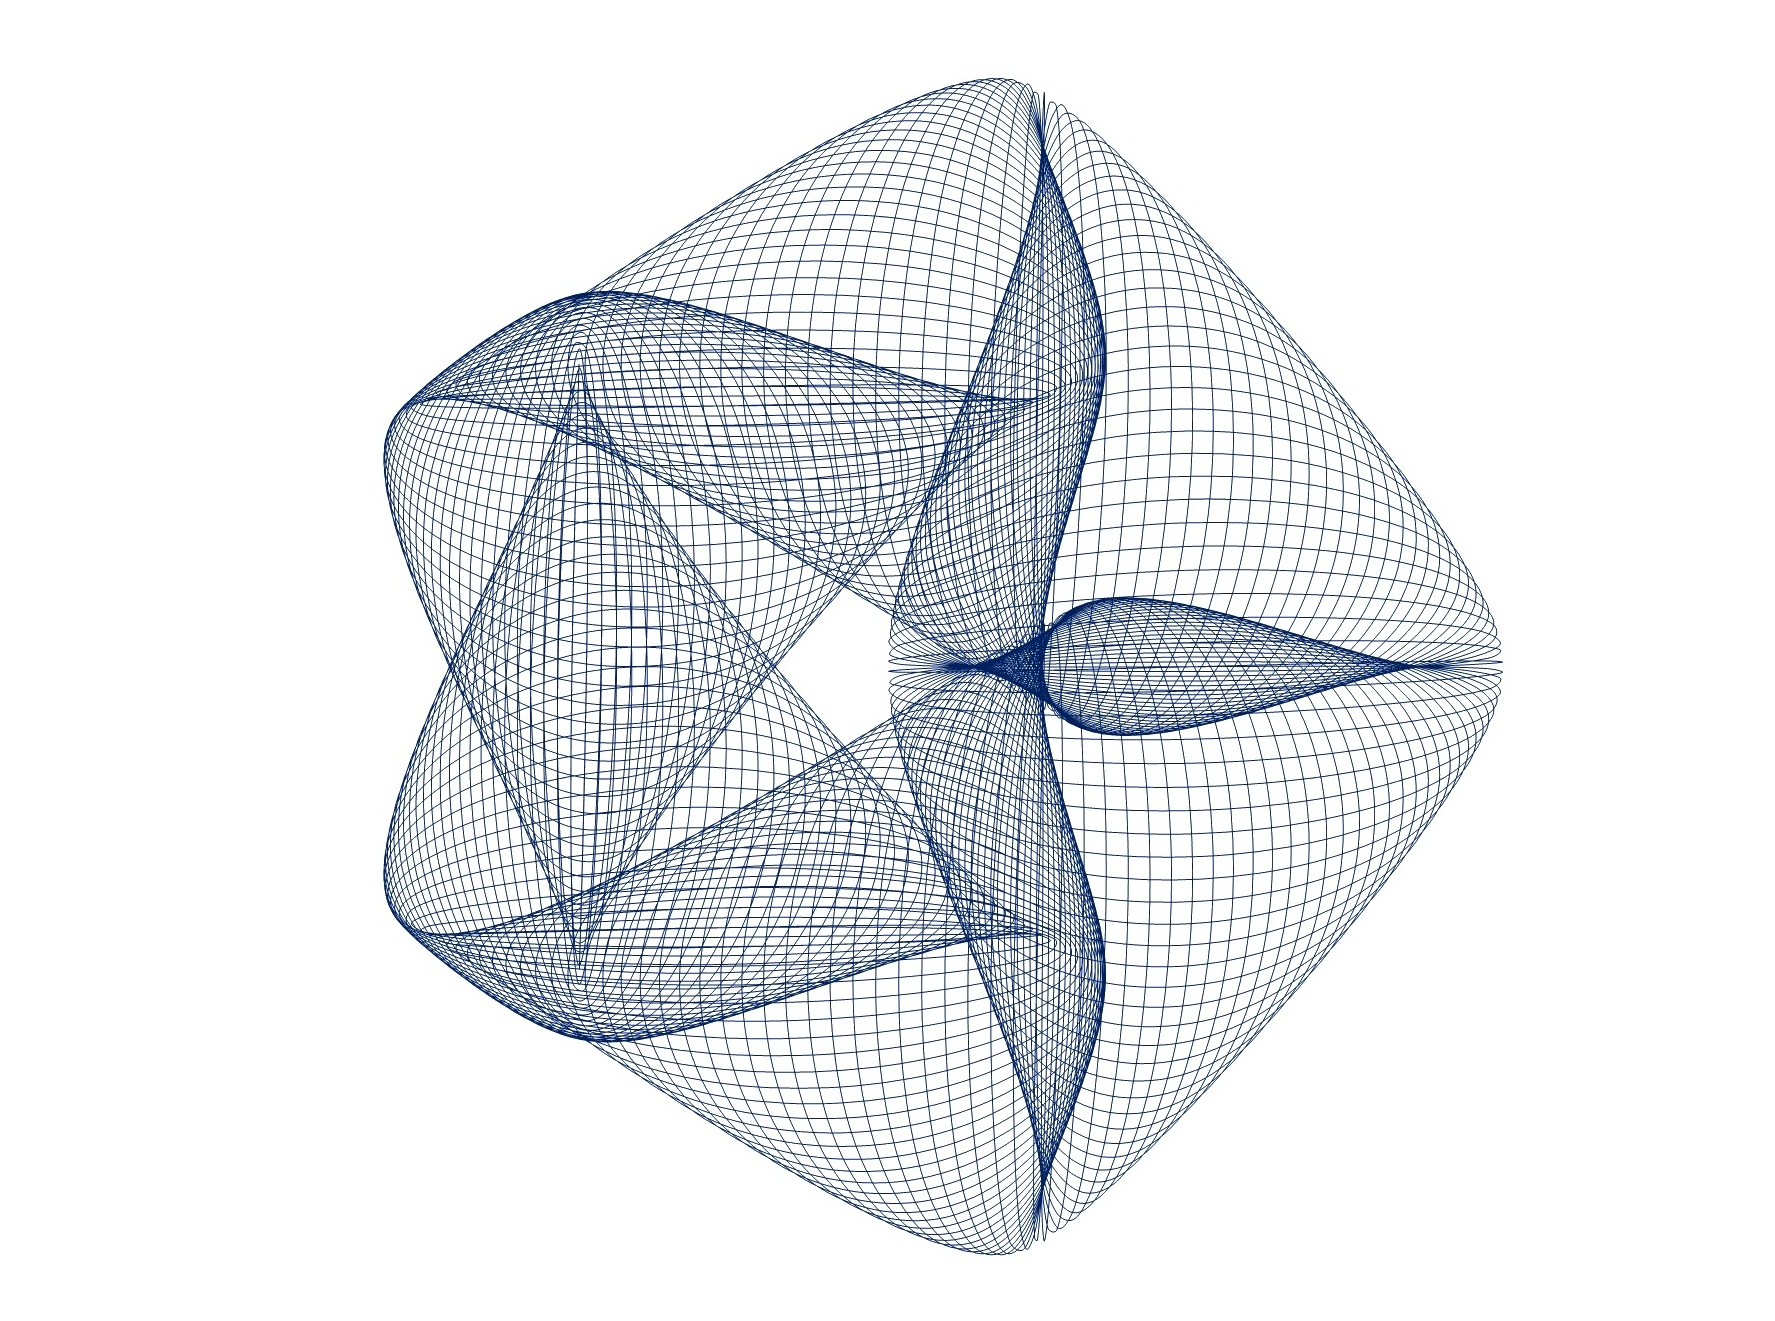
\includegraphics{../images/param_curve}}
    \end{figure}
\end{frame}

\begin{frame}[fragile]
    \frametitle{Flow perspectives}
    \begin{itemize}
        \item Function as flow
        \item Computation as flow, Effective flow
    \end{itemize}
    \begin{columns}
        \begin{column}{0.5\textwidth}
            \begin{center}
                \begin{tikzcd}
                    H && H \\
                    R && R
                    \arrow["l", from=1-1, to=1-3]
                    \arrow["\nu"', from=1-1, to=2-1]
                    \arrow["\nu", from=1-3, to=2-3]
                    \arrow["k"', from=2-1, to=2-3]
                \end{tikzcd}
            \end{center}
        \end{column}
        \begin{column}{0.5\textwidth}
            \begin{figure}[ht]\centering
            \resizebox{\textwidth}{!}{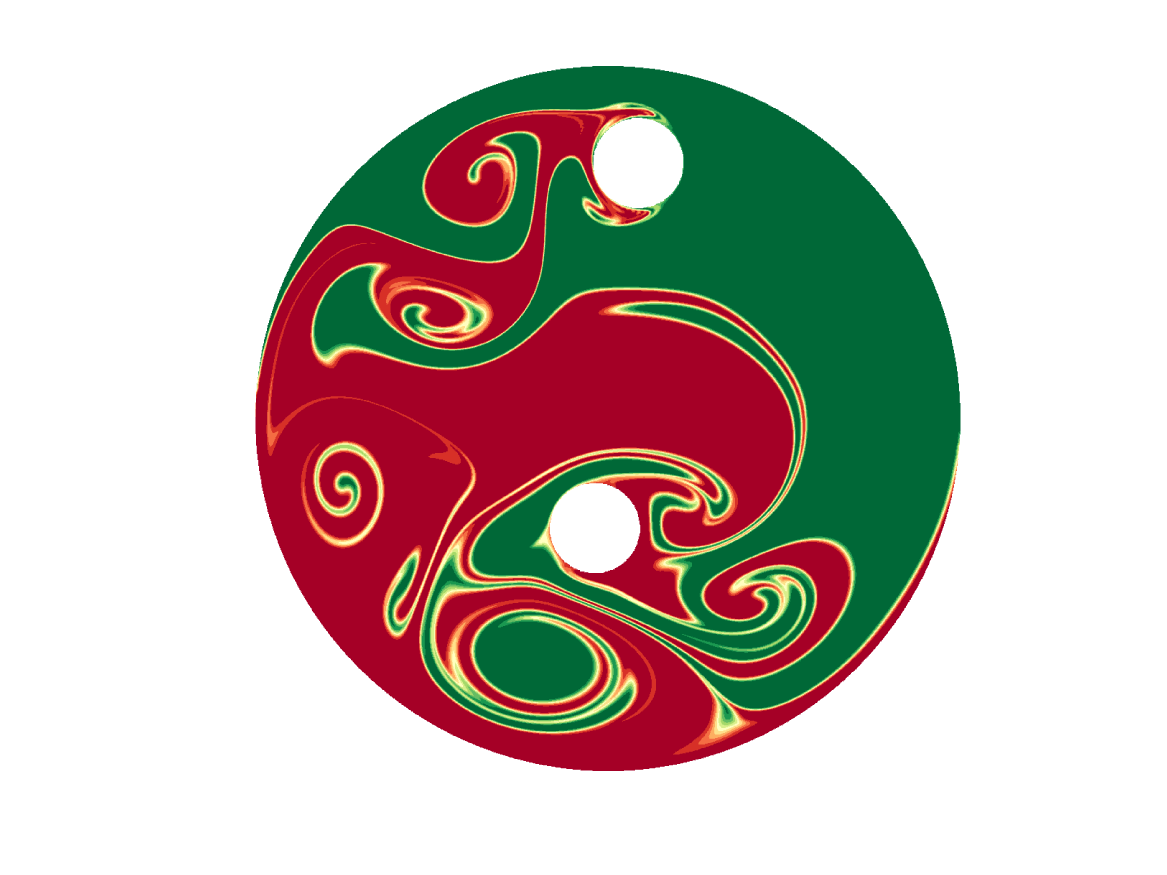
\includegraphics{../images/flow}}
            \end{figure}
        \end{column}
    \end{columns}
\end{frame}

\begin{frame}
    \frametitle{Binary numeral as effective flow}
    \begin{center}
        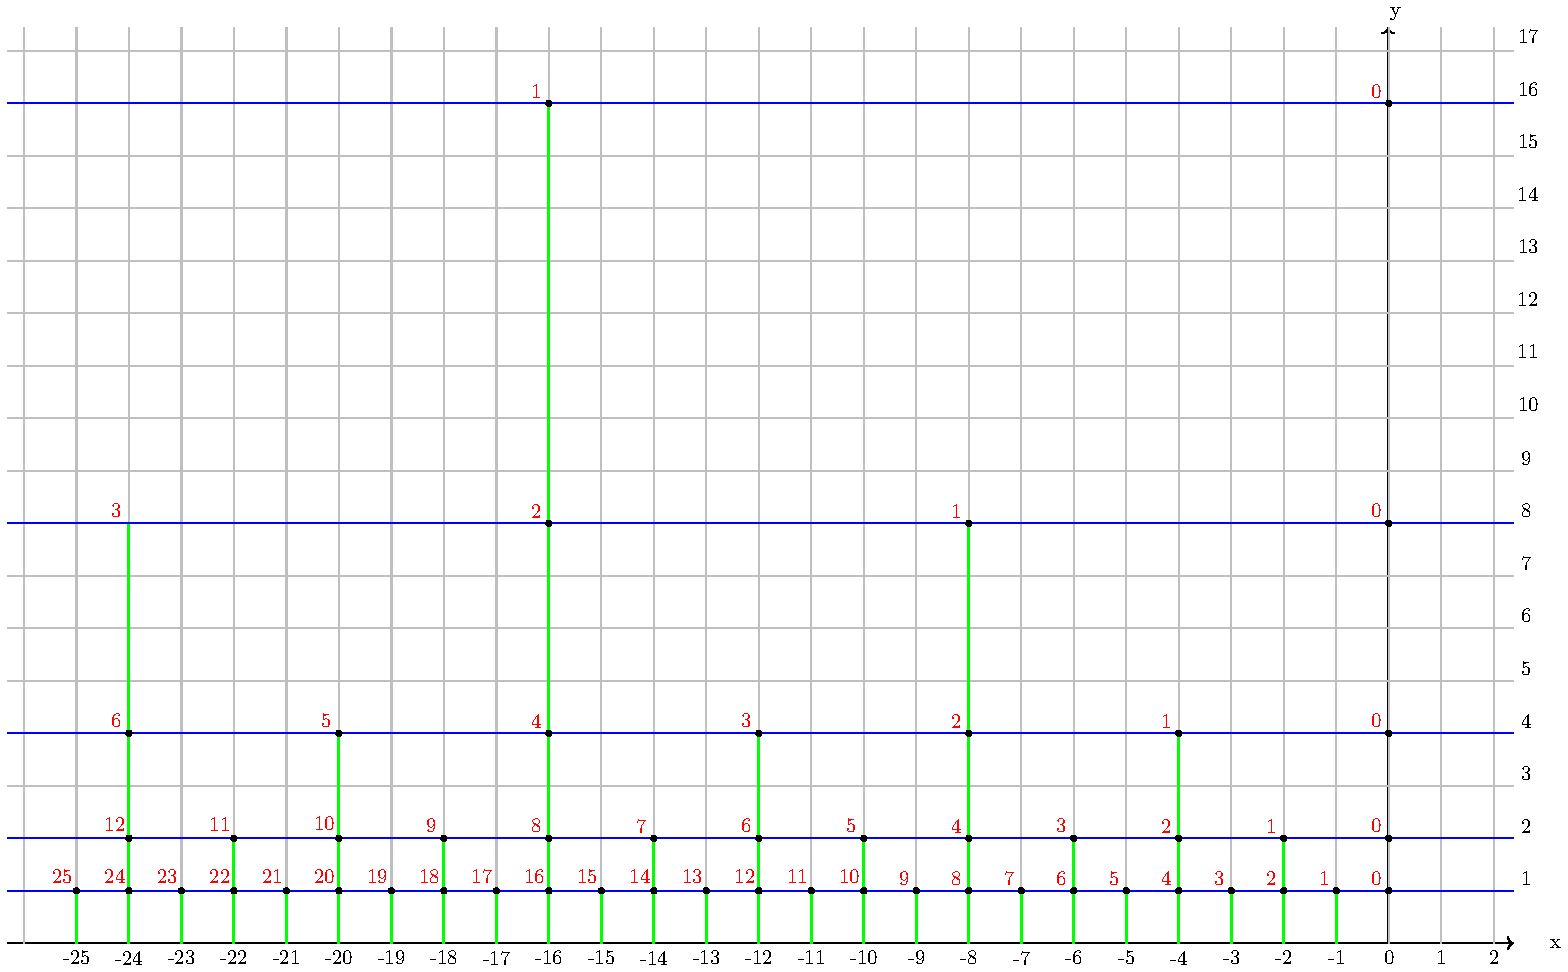
\includegraphics[width=0.6\textwidth]{../images/binarynumeral}
    \end{center}
\end{frame}

\begin{frame}
    \frametitle{Binary numeral as effective flow}
    We have
    \begin{center}
         $\frac{3}{2}_{10} = 1.1_{2}$,  $\frac{7}{4}_{10} = 1.11_{2}$ and $\frac{21}{8}_{10} = 10.101_{2}$.
        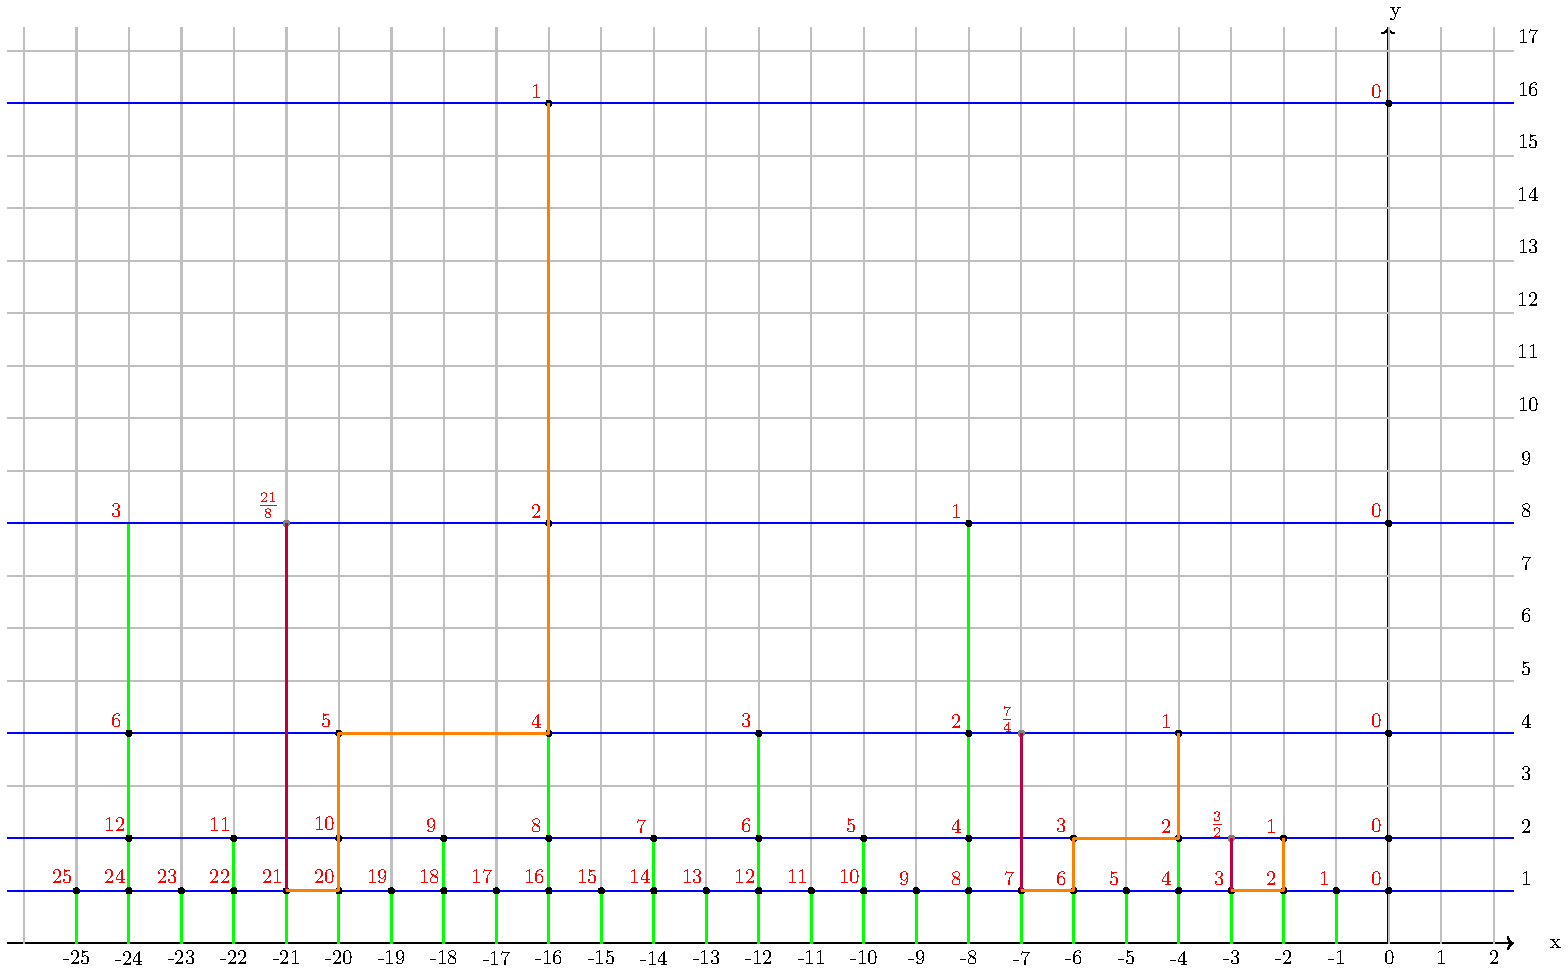
\includegraphics[width=0.7\textwidth]{../images/multiplication}
    \end{center}
\end{frame}

\begin{frame}
    \frametitle{Multiplication as effective flow?}
    Using multiplication as a case study, we should focus on the following questions:
    \begin{itemize}
        \item How to define the flow of multiplication?
        \item How to measure the time complexity of multiplication flow?
        \item How to measure the space complexity of multiplication flow?
    \end{itemize}
\end{frame}

\begin{frame}
    \frametitle{Space-time complexity?}
    The trade-off between space and time complexity is common in algorithm design,
    but the conversion between space and time complexity means they are the same thing from a conceptual perspective.
    We need study the trace of a computation process.
    AEG provides a testbed for this study.
\end{frame}

\section{Final remarks}

\begin{frame}
    \frametitle{Final remarks}
    \begin{enumerate}
        \item Grothendieck on triviality
        \item A kid's problem
    \end{enumerate}
\end{frame}

\begin{frame}
    \frametitle{Grothendieck on triviality}
    Alexander Grothendieck once emphasized the triviality in mathematics in his letter:
    \newline\newline
    \begin{center}
        \begin{quote}
            The difficulty of bringing new concepts out of the dark ...
        \end{quote}
    \end{center}
\end{frame}

\begin{frame}
    \frametitle{A kid's problem}
    Cake-cutting is a classic problem and studied in mathematics, computer science, economics and political science,
    and it is taught in primary school.

    One day, my kid asked me a question: "Why the more pieces I cut the more unfairness I get, if we use as less cut as possible?"
    \begin{figure}[ht]\centering
    \resizebox{0.5\textwidth}{!}{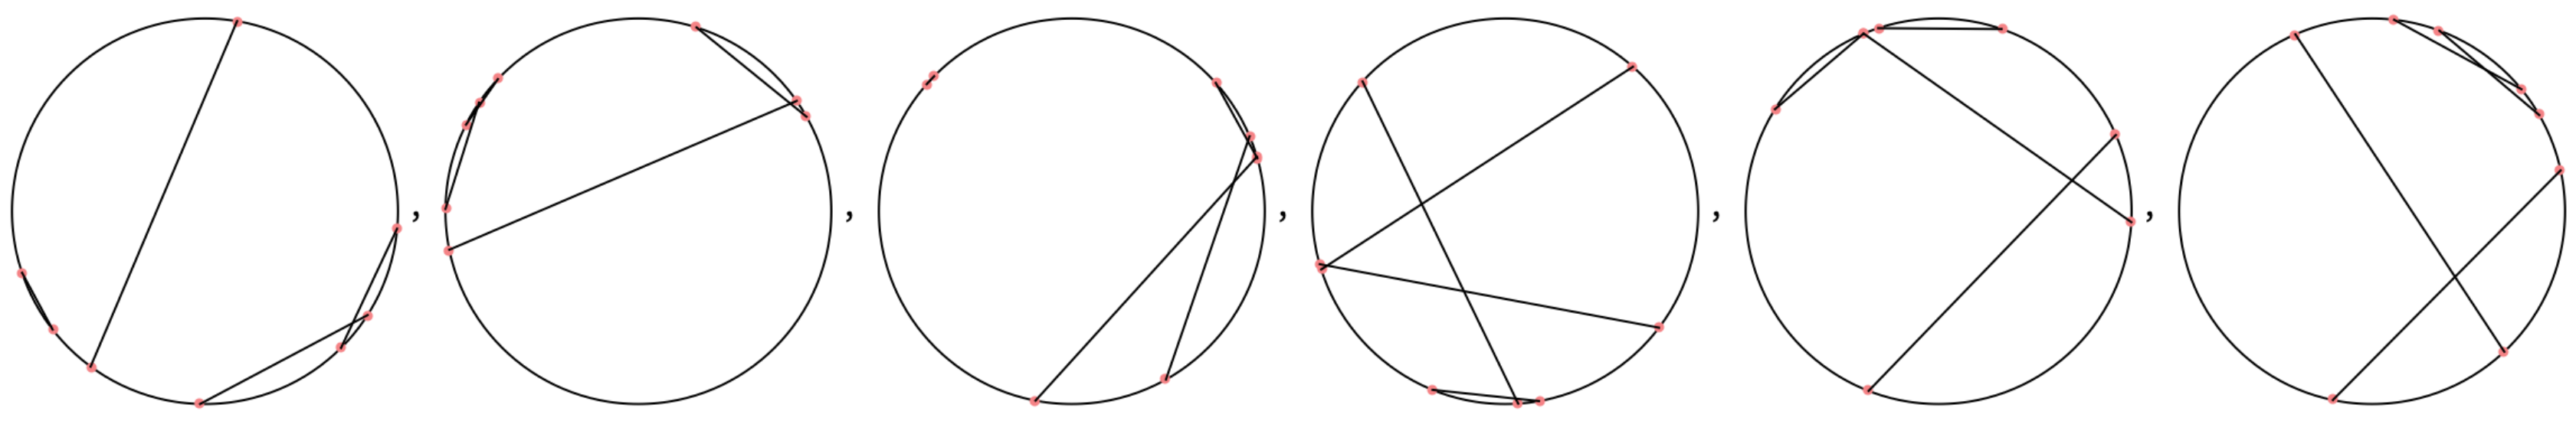
\includegraphics{../images/random-cuts}}
    \end{figure}
    We may introduce "area entropy" and "edge entropy" to measure the fairness of a cake-cutting, but what is the connection between
    the entropy and the number of cuts? What is the relationship between the "area entropy" and "edge entropy"?
\end{frame}

\begin{frame}
    \frametitle{Open to the unknown}
    Open your eyes as a kid, keep curiosity alive and mind open, and you will find the beauty of mathematics everywhere.
    \newline Thank you!
\end{frame}

\end{document}
